% Documentclass options:
%    10pt, 11pt, 12pt  -- set type size
%    draft             -- single space, mark overfull hboxes on paper
%    final             -- double space, don't mark overfull hboxes on paper
%    oneside           -- format for one-sided printing
%    twoside           -- format for two-sided printing
% Defaults are 11pt,final,oneside.  Keep these, please.
\documentclass[11pt]{ucscthesisbs}
\bibliographystyle{apalike2}
\usepackage{natbib}
\usepackage{graphicx,epsf}% Include figure files
\usepackage{spverbatim}
\newcommand{\aj}{Astronomical Journal}
\newcommand{\apj}{Astrophysical Journal}
\newcommand{\icarus}{Icarus}
\newcommand{\aap}{Astronomy and Astrophysics}     % Astronomy and Astrophysics 
\newcommand{\mnras}{Monthly Notices of the Royal Astronomical Society} 
\newcommand{\nat}{Nature} 
\newcommand{\jgr}{Journal of Geophysical Research}
 
% The following declaration is for citations and bibliographies consistent with
% Astrophysical Journal specifications.  It may be left out or replaced with
% another bibliography/citation style.  See also the "\bibliographystyle"
% command later in this file.
%\usepackage{apj}

\usepackage{xcolor}
\usepackage{pagecolor}
\usepackage{lipsum}  
\usepackage{subfig}
\usepackage{amsmath}
\usepackage[font=small,labelfont=bf]{caption}
\usepackage{mathabx}
\usepackage{stackengine}
\newcommand\xrowht[2][0]{\addstackgap[.5\dimexpr#2\relax]{\vphantom{#1}}}



% \pagecolor{darkgray}
% \color{white}

\pagecolor{white}
\color{black}


\begin{document}

% Declarations for Front Matter

\title{Thermal Evolution of Uranus and Neptune with Condensation-inhibited Convection}
\author{Robert Schroder}
\degreeyear{2021}
\degreemonth{March}
\degree{BACHELOR OF SCIENCE}
\field{ASTROPHYSICS}%

% Declare up to five committee members.  The text will be reproduced directly
% on the signature page.  Though the chair is a committee member, leave
% him/her out of the \committeemember declarations.  Make sure \numberofmembers
% agrees with the number of committee members declared INCLUDING the chair.
% If it is wrong, you will get extra or missing lines on the signature page.
%
\chair{Bruce Schumm}
\thesisadvisor{Christopher Mankovich}
\technicaladvisor{Jonathan Fortney}
\numberofmembers{2}




\campus{Santa Cruz}

\maketitle
\copyrightpage

\begin{frontmatter}

\begin{abstract}
Voyager 2 data appears to show that Uranus has no intrinsic flux. Contemporary, dry adiabatic models predict a warmer Uranus at present time. We examine under what conditions stable water condensation zones would form in the hydrogen dominated atmospheres of our solar system ice giants. We study these stable condensation zones in the context of an interior structure model that departs from conventional dry-adiabatic models by including a moist adiabatic interior. We investigate how stable water condensation zones impact the warming of the interior, and what impact the presence of these zones have on the thermal evolution of the ice giants. We find that the existence of stable water condensation zones do not explain Uranus's present luminosity anomaly. We also find that a moist adiabatic interior with the inclusion of stable water condensation zones result in a warmer Uranus and Neptune at present time than predicted by models with simple dry adiabatic or moist adiabatic interiors.
\end{abstract}

\tableofcontents
%
% The most recent (10/95) guidelines make absolutely no mention of the list
% of figures and list of tables.  Are they necessary?  If not, comment the
% next two lines out.
%
\listoffigures
% \listoftables


\end{frontmatter}

%\part{First Part}

\chapter{Introduction}
According to core accretion theory, planets coalesce from matter contained within their parent star's protoplanetary disk. A planet will accrete matter from the disk until the supply of matter has been exhausted, at which point, the planet will begin to cool and contract over time \citep{2007prpl.conf..591L,2013apf..book.....A}. It is natural to ask, what is a planet's temperature as it cools? Are we talking about the temperature at the surface? What do we mean by surface? How does energy get transported through the planet's interior? Does it conduct, convect, radiate, or all of these? If so, where, and under what conditions? Do clouds form, and do they impact a planet's cooling trajectory? These are some of the questions that physicists attempt to answer when modeling giant planet interiors and atmospheres. The sections in this first chapter will begin by reviewing some of thermodynamic concepts relevant to the physics of giant planet interiors, and will close with a brief overview of prior work on interior structure models that specifically motivated this work. In Chapter 2, we'll describe a conventional model for ice giant interior structure, and how our moist-convective model differs. We present our results in Chapter 3, describing where and when stable water condensation zones form, how they impact cooling within the interior, and their impact on thermal evolution. In Chapter 4, we discuss our conclusions and offer suggestions for future work.

\section{Relevant Thermodynamics}
\subsection{Temperatures}
There are several temperatures we are concerned with. Beginning with the effective temperature, $T_{\rm eff}$, which is defined in terms of the total power, $F_{P}$, leaving from each unit area of the surface of a blackbody \citep{pierrehumbert_2010}:
\begin{equation}
   F_{P} =  \pi \int_{0}^{\infty} B(\nu, T) d\nu = \sigma_{\rm B}T_{\rm eff}^{4},
  \label{eq:effective_temp_integral}
\end{equation}  
where $\sigma_{B}$ is the Stefan-Boltzmann constant, and $\nu$ is the frequency. Solving for $T_{\rm eff}$ yields
\begin{equation}
    T_{\rm eff} = \bigg(\frac{F_{\rm P}}{\sigma_{\rm B}}\bigg)^{\frac{1}{4}}.
  \label{eq:effective_temp}
\end{equation}

The equilibrium temperature, $T_{\rm eq}$, is the temperature the planet would have if it were in thermal equilibrium with its parent star. This occurs when the planet has radiated away its latent heat of formation, and the only remaining source of energy is from its star. This temperature\citep{seager_2010} is estimated as
\begin{equation}
    T_{\rm eq} = (T_{\rm eff\star})\bigg(\frac{R_{\star}}{a}\bigg)^{\frac{1}{2}}[f(1-A_{B})]^{\frac{1}{4}},
  \label{eq:equilibrium_temp}
\end{equation} 
where $T_{\rm eff\star}$ is the effective temperature of the parent star, $R_{\star}$ is the star's radius, and $a$ is the semi-major axis of the planet's orbit. The factor $(1 - A_{\rm B})$ is the the fraction of power from the parent star absorbed by the planet's atmosphere; here, the Bond albedo $A_{B}$ represents the fraction of the parent star's incident power that is reflected back into space. The factor $f$ accounts for the planet's distribution of the radiation it receives from its parent star. We make the assumption assumption that for Neptune and Uranus that the Sun's radiation is evenly distributed throughout, and thus $f = 1$. 

Finally, the intrinsic temperature, $T_{\rm int}$, is the temperature that defines the flux from the planet's interior and is defined by the relation

\begin{equation}
    T_{\rm eff}^4 =  T_{\rm eq}^4 +  T_{\rm int}^4.
  \label{eq:effective_temp}
\end{equation} 

\subsection{Means of Energy Transport}
How energy flows throughout a planet's interior impacts its actual vertical temperature structure, known as the temperature gradient, defined as
\begin{equation}
  \nabla_{T} = \frac{d \ln T}{d\ln P} ,
\end{equation}
where $T$ is temperature and $P$ is pressure. In this section, we'll review the relevant modes of energy transport within a giant planet's interior and discuss the criteria for convection and condensation to occur.

Convection is a common mode of energy transport in giant planet interiors. In this process, large-scale vertical temperature gradients drive kinetic fluid motions that carry heat toward the planet's surface. In the limit that parcels of the convective fluid do not exchange heat with their surroundings as they move, we describe the fluid motions as `adiabatic'. In this limit, the temperature profile follows a dry adiabatic gradient, or lapse rate \citep{kippenhahn_2012} given by
\begin{equation}
  \nabla_{\rm ad} = \left( \frac{\partial \ln T}{\partial \ln P} \right)_{\rm s},
  \label{eq:dry_lapse_rate}
\end{equation}
where $s$ is entropy. In the atmosphere, where the ideal gas law is valid, the vertical temperature structure can also be expressed in terms of temperature and altitude \citep{sanchez-lavega} as
\begin{equation}
  \frac{dT}{dz} = \frac{-g}{C_{P}} = \Gamma_{\rm dry},
\end{equation}
where $z$ is the altitude, and $C_{P}$ is specific heat at constant pressure. To determine whether a layer is dynamically unstable in a region of homogeneous chemical composition, we use the Schwarzschild \& Harm criterion \citep{kippenhahn_2012} as the criterion for convection, defined as
 \begin{equation}
  \nabla_{T} > \nabla_{\rm ad}.
\end{equation}
In a region that does not have a homogeneous chemical composition, but rather also has a gradient in mean molecular weight, defined as
 \begin{equation}
 \nabla_{\mu} = \frac{d \ln \mu}{d \ln P}, 
\end{equation}
 we use the Ledoux criterion\citep{kippenhahn_2012}
\begin{equation}
  \nabla_{T} > \nabla_{\rm ad} + \frac{\rho}{\delta}\nabla_{\mu},
  \label{eq:ledoux}
\end{equation}
where
\begin{equation}
  \rho = \bigg(\frac{\partial \ln \rho}{\partial \ln \mu}\bigg)_{P,T}
\end{equation}
and
\begin{equation}
 \delta = -\bigg(\frac{\partial \ln \rho}{\partial \ln T}\bigg)_{P,\mu}.
\end{equation}
The Ledoux criterion tells us that if the sum of the gradients on the right-hand side are less than the temperature gradient on the left, then the zone is dynamically unstable and convection occurs. Conversely, if $\nabla_{T} < \nabla_{\rm ad} + \frac{\rho}{\delta}\nabla_{\mu}$, then the region is stable, and convection is inhibited.

Condensation can also have a large impact on a planet's energy balance. For example, the presence of clouds can change a planet's albedo, impacting greatly the amount of radiation a planet receives from its star, or the amount of energy that the planet itself radiates away. The process of condensing vapor results in the release of energy, impacting the flow of energy through the interior. So, it is important consider the presence of condensible species when modeling the interior of giant planets. Gases condense at at sufficiently low temperatures or high pressures. Condensation of a gas is characterized by its saturation vapor pressure, which derives from the Clausius-Clapeyron equation \citep{sanchez_2011}. The saturation vapor pressure, $P_{\rm sat}$, is given by 
\begin{equation}
  P_{\rm sat}(T) = P_{\rm sat}(T_{\rm 0})e^{-\frac{L + C_{\rm p}T_{\rm 0}}{R_{\rm vap}}(\frac{1}{T} - \frac{1}{T_{\rm 0}}) -\frac{C_{\rm p}}{R_{\rm vap}}\ln{\frac{T}{T_{\rm 0}}}}
  \label{eq:saturation_vapor_pressure}
\end{equation}{}
where $T_{\rm 0} = 273.16$ K, and $R_{\rm vap}$ is the gas constant for the condensible species, and $L$ is the latent heat of vaporization for the condensate. When the partial pressure of a gas, $P_{\rm gas}$, is less than $P_{\rm sat}$, the parcel of gas is `subsaturated'. When $P_{\rm gas} = P_{\rm sat}$, the gas is `saturated'. And, when $P_{\rm gas} > P_{\rm sat}$, the parcel is `supersaturated'. Every condensible species has its own saturation vapor pressure. We assume a single condensible species and calculate the moist adiabat as \citep{sanchez_2011} 
\begin{equation}
  \nabla_{\rm moist} = 1 + \frac{\frac{x_{\rm vap} L}{R_{\rm vap}T}}{\nabla_{\rm ad} + \frac{L^2}{R_{\rm vap}^2 T^2}}.
  \label{eq:moist_lapse_rate}
\end{equation}
It is important to recognize that the moist adiabatic lapse rate, Equation \ref{eq:moist_lapse_rate}, is less than the dry adiabatic lapse rate given by Equation \ref{eq:dry_lapse_rate}. The reason for this is that condensation of vapor releases latent heat. This latent heat release boosts convection, but it also offsets adiabatic cooling. This situation becomes a more nuanced when we encounter gradients in mean molecular weight in the next section. Finally, we assume that the condensation zones are at saturation so that the vapor mole fraction, $x_{\rm vap}$, is equal to the saturation vapor mole fraction:
\begin{equation}
x_{\rm vap} = x_{\rm vap}^{\rm sat} = \frac{P_{\rm sat}}{P}, \qquad P_{\rm top} < P < P_{\rm base}.
\end{equation}

Condensation on Earth is notably different from condensation that occurs in hydrogen dominated atmospheres. On Earth, and the ice giants, as a parcel of air is lifted, it cools until it gets cold enough that water vapor condenses out, releasing latent heat. This release of energy alters the temperature-pressure profile of the atmosphere, which now follows a moist adiabat. But, in addition to altering the temperature gradient, condensation also creates a gradient in mean molecular weight. For example, on Earth, moist air is lighter than dry air. H$_{2}$O vapor (molecular mass = 18 g/mol), the primary condensate in Earth's atmosphere, is lighter than the background air which is composed primarily of N$_{2}$ (molecular mass = 28 g/mol). When H$_{2}$O vapor abundance exceeds the saturation vapor pressure, the excess vapor condenses out of the atmosphere, resulting in a vertical gradient in mean molecular weight. Since the condensate (water) is lighter than the background gas, rainout leads to a destabilized, top-heavy parcel allowing the parcel to turn over which further aids convection. By contrast, in the hydrogen dominated atmospheres of Neptune and Uranus, the background gas is much lighter than the condensate (water). Thus, when condensation occurs, the rainout of H$_{2}$O creates a bottom-heavy parcel, leading to a gradient in mean molecular weight that is opposite in sign to the gradient we encountered with the scenario for Earth. This bottom-heavy gradient in mean molecular weight can have a stabilizing effect on the rising parcel of gas, resulting in a situation where the zone is stable against convection \citep{guillot_1995,friedson_2017,leconte_2017}. 

It is important to highlight that we have been discussing H$_{2}$O as the only condensate. However, other condensates such as NH$_{3}$ and CH$_{4}$ may impact convection as well. In this study, we only consider H$_{2}$O as the primary condensate since oxygen is the most plentiful atomic species following H and He \citep{leconte_2017}. As pointed out by \citep{guillot_1995}, an oxygen abundance greater than ten times solar would be sufficient to inhibit convection on Jupiter, Saturn, Uranus, and Neptune. This abundance is possibly an order of magnitude smaller than the expected enrichment for Uranus and Neptune \citep{2016arXiv160604510A}. If H$_{2}$O's abundance is supercritical, it results in a larger superadiabicity (larger temperature gradient) than would be provided by either NH$_{3}$ or CH$_{4}$ \citep{guillot_1995}. We therefore prioritize H$_{2}$O condensation for this work and leave the effect of other condensates for future study. 


\section{Prior Work}
In 1965, Frank Low measured Jupiter's intrinsic temperature \citep{low_1966}. To explain this observation, theorists \citep{hubbard_1968, smoluchowski_1967,hubbard_1977, hubbard_1977_2, podolak_1991} set out to expand on the seminal work by \citep{demarcus_1958} on the theory of interior structure of solar system giant planets. In 1968, it was Hubbard who showed that a convective interior would allow Jupiter's observed flux to be transported to the surface adiabatically. This analysis motivated the inclusion of dry adiabatic interiors in contemporary interior structure models for gas and ice giants.

At the present time, most of the giant planets in our solar system: Saturn, Jupiter, and Neptune, all have an observed intrinsic flux. Uranus is the exception \citep{pearl_conrath_1991}. Measurements of Uranus's effective temperature are consistent with a planet that has no intrinsic flux, a planet in thermal equilibrium with the Sun, cooler than its more distant neighbor, Neptune, a planet of similar mass and composition. The observed $T_{\rm eff}$, $T_{\rm eq}$, and internal energy flux for the giant planets are listed in Table \ref{tab:planetary_temperatures}.
\renewcommand{\arraystretch}{1.5}
\begin{table}[h]
\centering
\begin{tabular}{lllll}
Parameter                                                               & Jupiter                              & Saturn                               & Uranus                                 & Neptune                              \\ \hline
\multicolumn{1}{|l|}{$T_{\rm eq}$ (K)}                                  & \multicolumn{1}{l|}{$109.5 \pm 1.4$} & \multicolumn{1}{l|}{$82.4 \pm 0.9$}  & \multicolumn{1}{l|}{$58.2 \pm 1.0$}    & \multicolumn{1}{l|}{$46.2 \pm 0.6$}  \\ \hline
\multicolumn{1}{|l|}{$T_{\rm eff}$ (K)}                                 & \multicolumn{1}{l|}{$124.4 \pm 0.3$} & \multicolumn{1}{l|}{$95.0 \pm 0.4$}  & \multicolumn{1}{l|}{$59.1 \pm 0.3$}    & \multicolumn{1}{l|}{$59.1 \pm 2.0$}  \\ \hline
\multicolumn{1}{|l|}{Internal Energy Flux $(10^{-4} \frac{\rm W}{\rm cm^{2}})$} & \multicolumn{1}{l|}{$5.44 \pm 0.43$} & \multicolumn{1}{l|}{$2.01 \pm 0.14$} & \multicolumn{1}{l|}{$0.042 \pm 0.047$} & \multicolumn{1}{l|}{$0.43 \pm 0.09$}  \\ \hline
\end{tabular}
\caption{Temperatures of giant planets. The internal energy flux of Uranus is consistent with zero within the observational uncertainty. Table adapted from \citep{pearl_conrath_1991}}
\label{tab:planetary_temperatures}
\end{table}
\renewcommand{\arraystretch}{1}
While thermal evolution models do currently reproduce $T_{\rm eff}$ for Jupiter and Neptune at 4.6 Gyr \citep{graboske_1975,fortney_2011}, they do not reproduce $T_{\rm eff}$ for Saturn and Uranus. Models for Saturn predict a cooler planet; however, plausible explanations have been offered to explain its current, warmer $T_{\rm eff}$. Among them are the rain-out of helium \citep{fortney_hubbard_2003, 2020ApJ...889...51M}, or double-diffusive convection \citep{leconte_chabrier_2013}. 

Meanwhile, for Uranus, contemporary models have predicted a warmer effective temperature at present time \citep{fortney_2011, podolak_1991, hubbard_1995, 2019A&A...632A..70S}. There have been various attempts to explain Uranus's luminosity anomaly. Early investigations posited that a stratified interior, stable against convection, would allow heat to be trapped deep within the interior \citep{podolak_1991}. Later work investigated some other possible explanations for Uranus's cool temperature. \citep{guillot_1995} posited that condensates such as NH$_{3}$, CH$_{4}$, or H$_{2}$O when at critical abundance could interfere with convection, producing temperature profiles that would be superadiabatic. \citep{nettelmann_2016} looked at the inclusion of ad-hoc thermal boundary layers within a planet's interior and found that they could possibly explain Uranus's current $T_{\rm eff}$. \citep{friedson_2017,leconte_2017} explored the impact of condensates forming stable radiative layers. Both carried out linear stability analyses and reached similar findings, concluding that super-critical abundances of H$_{2}$O would result in a superadiabatic temperature gradient. All of these investigations showed that the presence of thermal boundary layers could possibly provide a mechanism to trap heat deep within the interior, allowing the envelope above to cool more rapidly.

The work done by \citep{guillot_1995,friedson_2017,leconte_2017} examined under what conditions stable condensation zones would form in hydrogen dominated atmospheres. In this paper, we apply the same physical mechanisms for the formation of stable water condensation zones. However, we expand on this by placing these stable, radiative layers in the context of a more complete model of interior structure for solar system ice giants. Finally, we investigate how these stable layers impact the cooling of the planets over time. 


\chapter{Model}

\section{Differential Equations for Structure and Evolution}
\label{Three-layer Model with Dry Adiabat}
We begin our description of the physics of our interior structure model by assuming that we are dealing with a spherically symmetric object with no electromagnetic field.  With these assumptions in place, we employ the following equations to describe the interior and evolution of ice giants.
\subsubsection{Conservation of Mass}
\begin{equation}
  \frac{dm}{dr} =4 \pi r^{2}\rho  ,
\end{equation}
where $dm$ is the mass contained between a sphere of radius $r$ and a sphere of of radius $r + dr$, and $\rho$ is the density. 
\subsubsection{Hydrostatic Equilibrium}
\begin{equation}
  \frac{dP}{dr} = -\frac{Gm\rho}{r^{2}}  ,
\end{equation}
where $P$ is the pressure and $G$ is the gravitational constant. 
\subsubsection{Conservation of Energy}
Conservation of energy implies that the planet's intrinsic luminosity, $L = 4\pi R^2\sigma_{B}T_{\rm int}^4$, 
must be balanced by the rate of change of its total internal energy. When we have a sequence of progressively cooler models, we calculate the time-step between any two models using the energy conservation equation as in \citep{fortney_2011}
\begin{align}
\frac{dL}{dm}= -T\frac{\partial S}{\partial t},
\label{eq:energy_conservation}
\end{align}
where $dm$ is the mass of the shell, $\partial S$ is the entropy of the shell, and $T$ is the temperature of the shell. Integrating over the mass and solving for $\partial t$, we get the time-step
\begin{equation}
\partial t = -\frac{1}{L} \int_{0}^{M} \partial S \,dm .
\label{eq:timestep}
\end{equation}

\section{Standard Interior Structure Model}
\subsubsection{Inputs}
We employ a three-layer interior structure, seen in the diagram on the left in Figure \ref{fig:standard_dry_interior}. 
\begin{figure}[ht!]
 \centerline{
  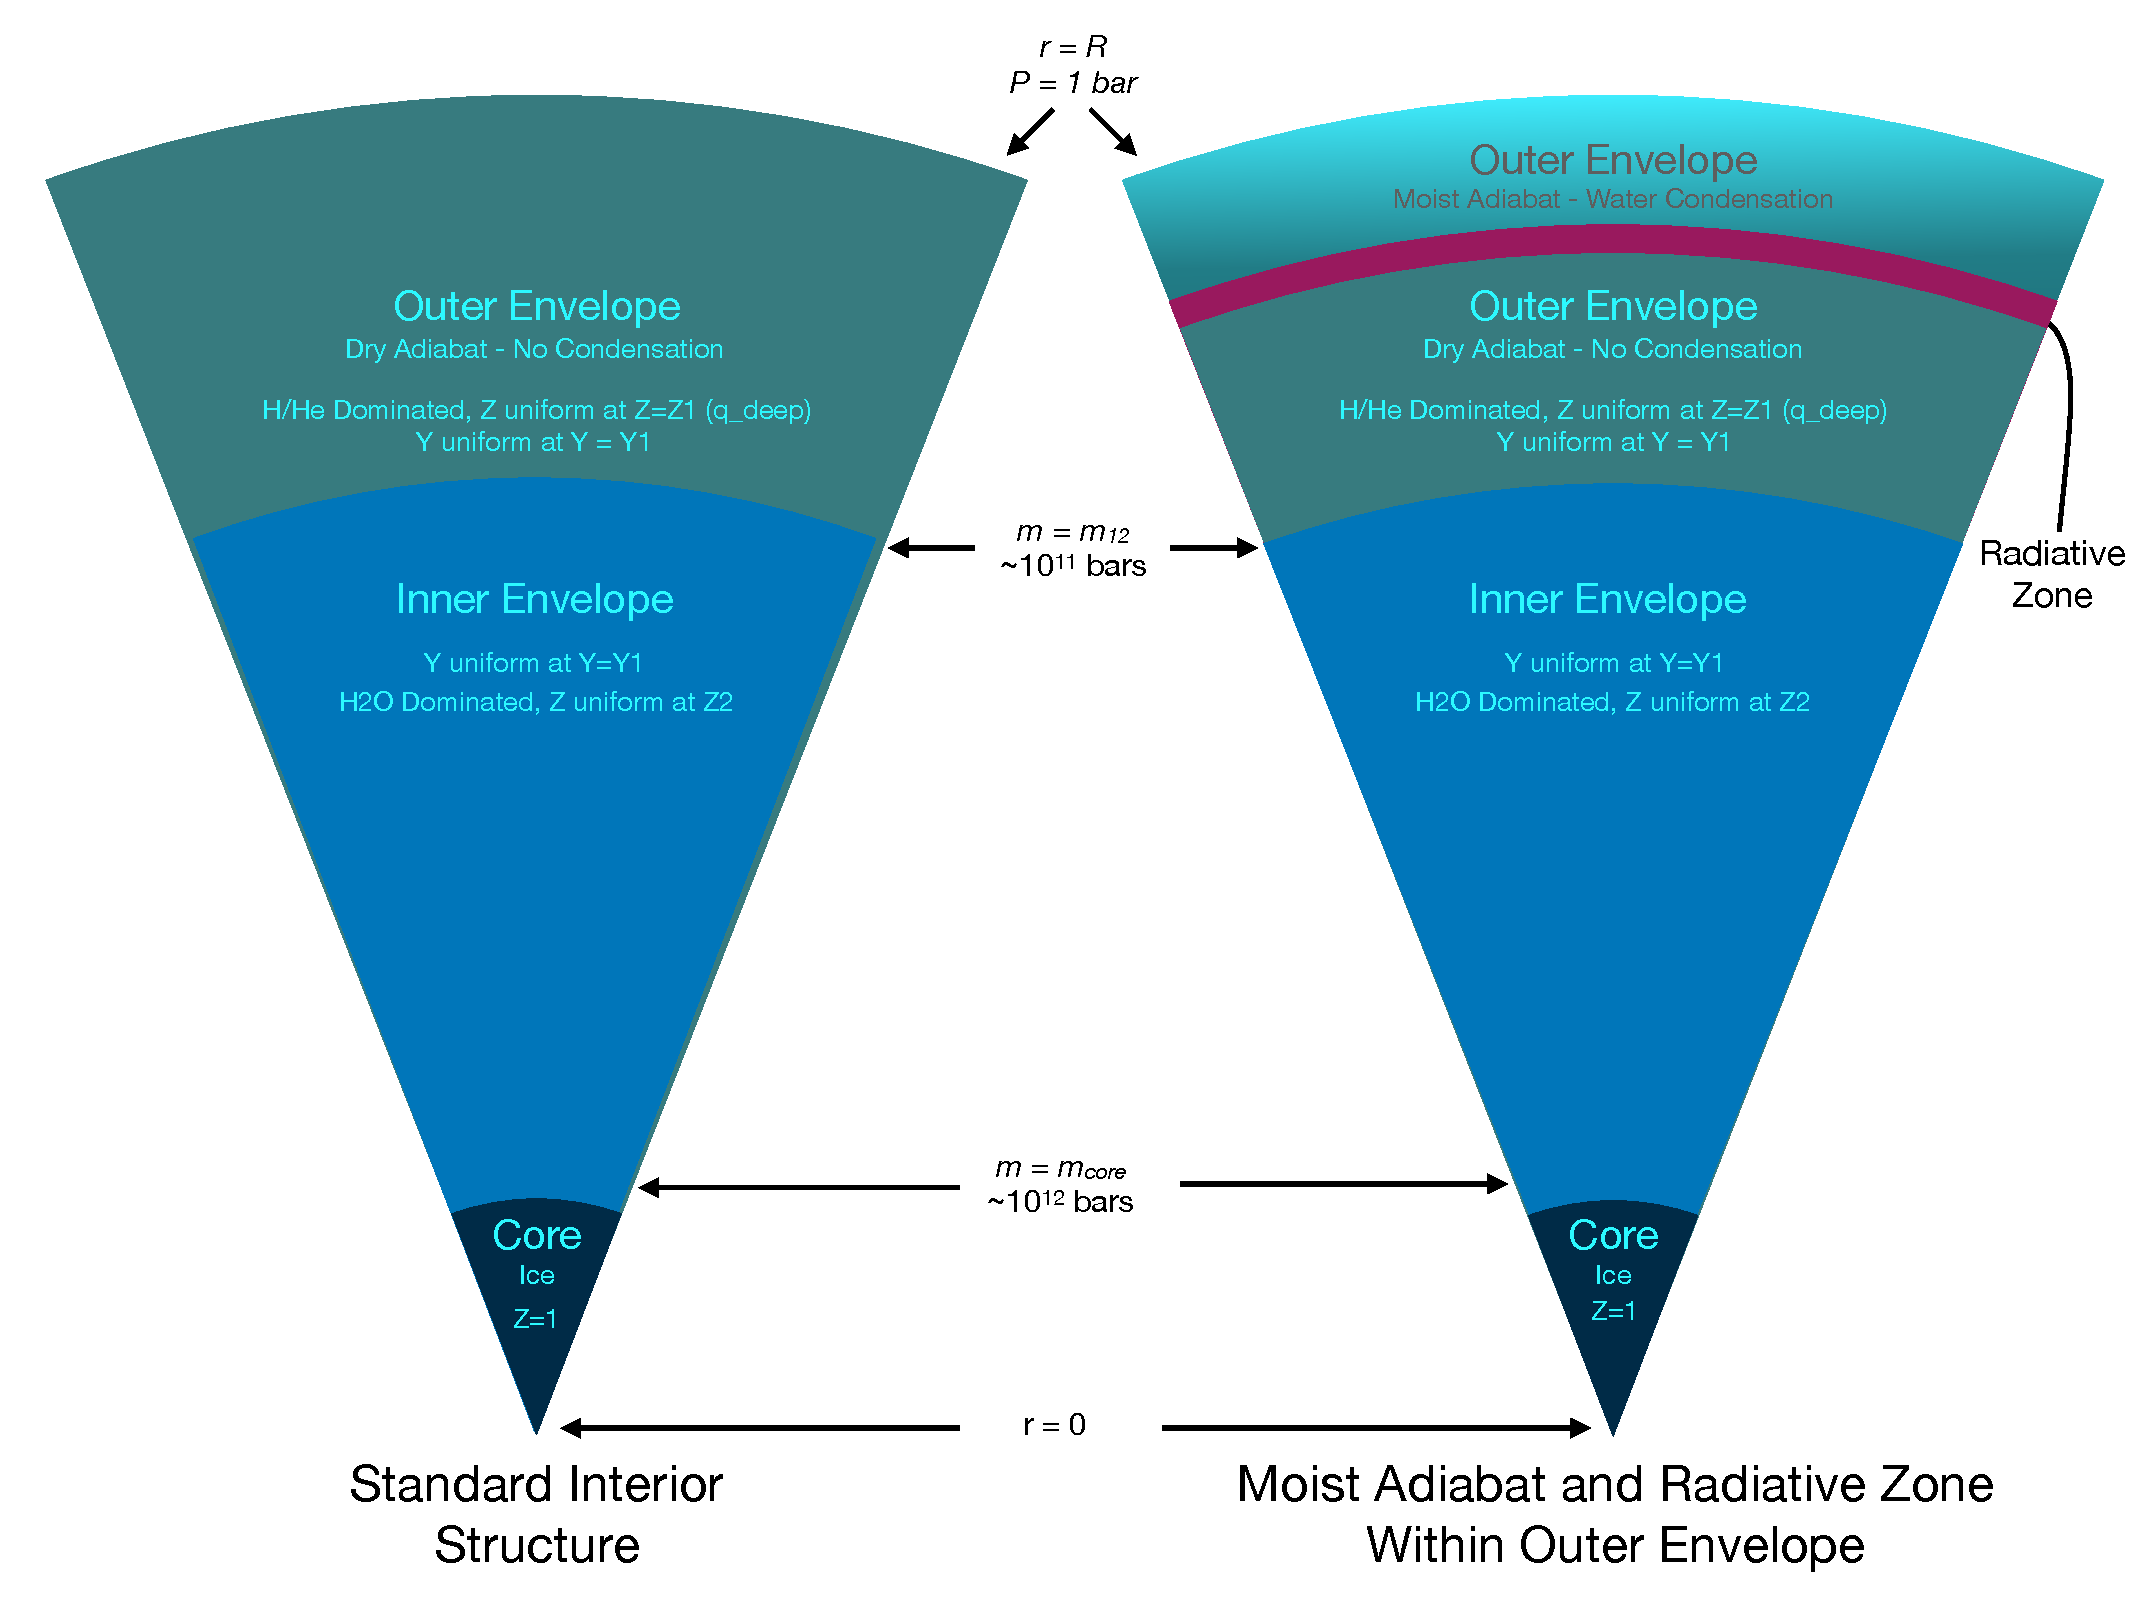
\includegraphics[width=\columnwidth]{figures/onion.pdf}
 }
\caption[A Standard Interior Structure Model]
{Comparison of interior structures. On the left: A conventional interior structure. In this interior structure model, the inner and outer envelopes are assumed to be well mixed, fully convective, and following a dry adiabat. The core is composed of water ice. The inner envelope is water dominated, with uniform concentrations of hydrogen, helium, and water; whereas, the outer envelope is hydrogen and helium dominated with trace amounts of water. The atmosphere extends beyond 1 bar, but pressures down to 1 bar are sufficient to capture the formation and impact of the water condensation zones investigated here. On the right: The the interior structure for moist adiabatic interior, allowing for interruption of convection. In this model, a stable water condensation zone may form. The red layer indicates the stable radiative layer. The pressure and temperature at the base of the radiative layer is set by the condition that $x_{\rm vap}$ has reached the deep value $x_{\rm vap}^{\rm deep}$. Below the condensation zone, the temperature and pressure follow a dry adiabat.}
\label{fig:standard_dry_interior}
\end{figure}
Broadly speaking, we assume a water `ice' core. There is an inner envelope that is composed mostly of H$_{2}$O, with trace amounts of H and He. We have left out other ices such as NH$_{3}$ and CH$_{4}$. The outer envelope is dominated by hydrogen and helium, with trace amounts of water, excluding methane and ammonia. It should be noted, that the concentration of ices in the interior of Neptune and Uranus is poorly constrained. These planets have not received the same amount of detailed observation from probes as have Jupiter and Saturn. As such, our model inputs assume a range of deep water concentrations within the outer envelope, from here on referred to as $q_{\rm deep}$. Furthermore, the mass fraction of H$_{2}$O in the inner envelope, $Z_{2}$, is also poorly constrained but can be estimated using models that fit Uranus's or Neptune's observed radii; see discussion in Section 3.3. The inputs to the model are tabulated in Tables \ref{tab:core_mass_and_inner_envelope_mass_fractions} and \ref{tab:outer_envelope_mass_fractions}.
\begin{table}[h]
\centering
\begin{tabular}{cccccc}
                              &                                                  &                                   &                              &                               \\ \hline
\multicolumn{1}{|c|}{Planet}  & \multicolumn{1}{c|}{$m_{\rm core}$}              & \multicolumn{1}{c|}{$m_{\rm 12}$} & \multicolumn{1}{c|}{$Y_{2}$} & \multicolumn{1}{c|}{$Z_{2}$}  \\ \hline
\multicolumn{1}{|c|}{Uranus}  & \multicolumn{1}{c|}{$1.51 m_{\Earth}$}           & \multicolumn{1}{c|}{12.5}         & \multicolumn{1}{c|}{0.03294} & \multicolumn{1}{c|}{0.87800}  \\ \hline
\multicolumn{1}{|c|}{Neptune} & \multicolumn{1}{c|}{$2.85 m_{\Earth}$}           & \multicolumn{1}{c|}{15.0}         & \multicolumn{1}{c|}{0.03996} & \multicolumn{1}{c|}{0.85200}  \\ \hline
\end{tabular}
\caption{Model inputs for the core and inner envelope. $m_{\rm core}$ is the core mass in units of Earth masses. $m_{\rm 12}$ is the mass coordinate for the boundary between the inner and outer envelope. $Y_{2}$ and $Z_{2}$ are the mass fractions for He and H$_{2}$O, respectively. The hydrogen mass fraction is found from $X_{2} = 1 - Y_{2} - Z_{2}$}
\label{tab:core_mass_and_inner_envelope_mass_fractions}
\end{table}
\begin{table}[h]
\centering
\begin{tabular}{ccccccc}
                              & $q_{\rm deep = 0.05}$         & $q_{\rm deep = 0.15}$         &  $q_{\rm deep = 0.25}$        \\ \hline
\multicolumn{1}{|c|}{Planet}  &  \multicolumn{1}{c|}{$Y_{1}$} &  \multicolumn{1}{c|}{$Y_{1}$} &  \multicolumn{1}{c|}{$Y_{1}$} \\ \hline
\multicolumn{1}{|c|}{Uranus}  &  \multicolumn{1}{c|}{0.2565}  & \multicolumn{1}{c|}{0.2295}   &  \multicolumn{1}{c|}{0.2025}  \\ \hline
\multicolumn{1}{|c|}{Neptune} &  \multicolumn{1}{c|}{0.2565}  &  \multicolumn{1}{c|}{0.2295}  &  \multicolumn{1}{c|}{0.2025}  \\ \hline
\end{tabular}
\caption{Model inputs for the outer envelope. $q_{\rm deep}$ is the deep water concentration. $Y_{1}$ is the He mass fraction. $q_{\rm deep} = Z_{1}$ and with the inner envelope mass fractions, $X_{1} = 1 - Y_{1} - Z_{1}$ }
\label{tab:outer_envelope_mass_fractions}
\end{table}
\subsubsection{Equations of State}
Near the surface, the ideal gas law provides a good approximation for relating pressure, temperature, density, and composition. However, at depth where pressures can be on the order of $10^{11}$ to $10^{12}$ bars, this approximation is no longer valid. We use \citep{chabrier_eos} as our H-He equation of state. For water, we use the \citep{mazevet_2019} EOS. 

\subsubsection{Relative Mass Abundances Within Each Layer}
$X$, $Y$, and $Z$ represent mass fractions for hydrogen, helium, and water, respectively. In general
\begin{equation}
  X + Y + Z = 1 .
\end{equation}
$Y'$ is the He mass fraction relative to He $+$ H, such that
\begin{equation}
  Y' = \frac{Y}{X+Y}.
\end{equation}
Referring to Figure \ref{fig:standard_dry_interior}, the center of the planet has a core of mass, $m_{\rm core}$. The core is made of pure water ice, indicated by $Z = 1$, the H$_{2}$O mass fraction. Moving outward, the inner envelope is H$_{2}$O dominated, with $Y_{2}$ and $Z_{2}$ representing the mass fractions of He and H$_{2}$O, respectively. The outer envelope's extent ranges from $P=1$ bar down to the outer-inner envelope boundary. The transition between the outer and inner envelopes is at a fixed mass coordinate $m_{12}$. The outer envelope contains trace amounts of H$_{2}$O and is mostly comprised of hydrogen and helium, with mass fractions equal to $X_{1}$ and $Y_{1}$, respectively. $T_{1}$ is the temperature at $P=1$ bar. 

We use the additive-volume approximation to determine total density, given by the relation
\begin{equation}
  \frac{1}{\rho} = \frac{X}{\rho_{\rm H}} + \frac{Y}{\rho_{\rm He}} + \frac{Z}{\rho_{\rm H_{2}O }}.
\end{equation}
Internal energy, $u$, is given by
\begin{equation}
 u = (X)(u_{\rm H}) + (Y)(u_{\rm He}) + (Z)(u_{\rm H_{2}O}),
\end{equation}
where $\rho_{\rm H}$ and $u_{\rm H}$ are the density and internal energy per gram of pure hydrogen at a given $P$, $T$. Quantities are defined similarly for helium and water.

\subsubsection{Atmospheric Boundary Condition}
Since atmospheres regulate how quickly the energy within a planet's interior can radiate into space, it is important to include a realistic atmospheric boundary condition as part of the interior structure model, as it provides key inputs that impact cooling times for the interior structure model and its evolution \citep{1975ApJ...199..265G,fortney_2011}. Specifically, the atmospheric boundary condition allows us to link the planet's $T_{\rm int}$ and $T_{\rm eff}$ to the model's surface gravity, $g$, and its $T_{1}$ (temperature at $P = 1$ bar) or $T_{10}$ (temperature at $P = 10$ bar). Our work utilizes the \citep{fortney_2011} model atmosphere which utilizes properties specific to solar system giants such as chemical abundance within the atmosphere, and incident flux as a function of the age of the solar system. 

\section{Inclusion of Moist Adiabat Within Outer Envelope of Standard Model}
Our interior structure model modifies the conventional structure described in Section \ref{Three-layer Model with Dry Adiabat} by allowing for moist convection within the outer envelope, as seen in the right-hand diagram in Figure \ref{fig:standard_dry_interior}. Under favorable conditions, the model allows for condensation of H$_{2}$O, and possibly the formation of a stable radiative layer that inhibits large-scale convection. To get a sense for how moist convection, or the presence of a stable radiative layer can alter the vertical temperature structure of a planet's interior, we refer to Figure \ref{fig:comparison_adiabatic_profiles}. 
\begin{figure}[h]
 \centerline{
  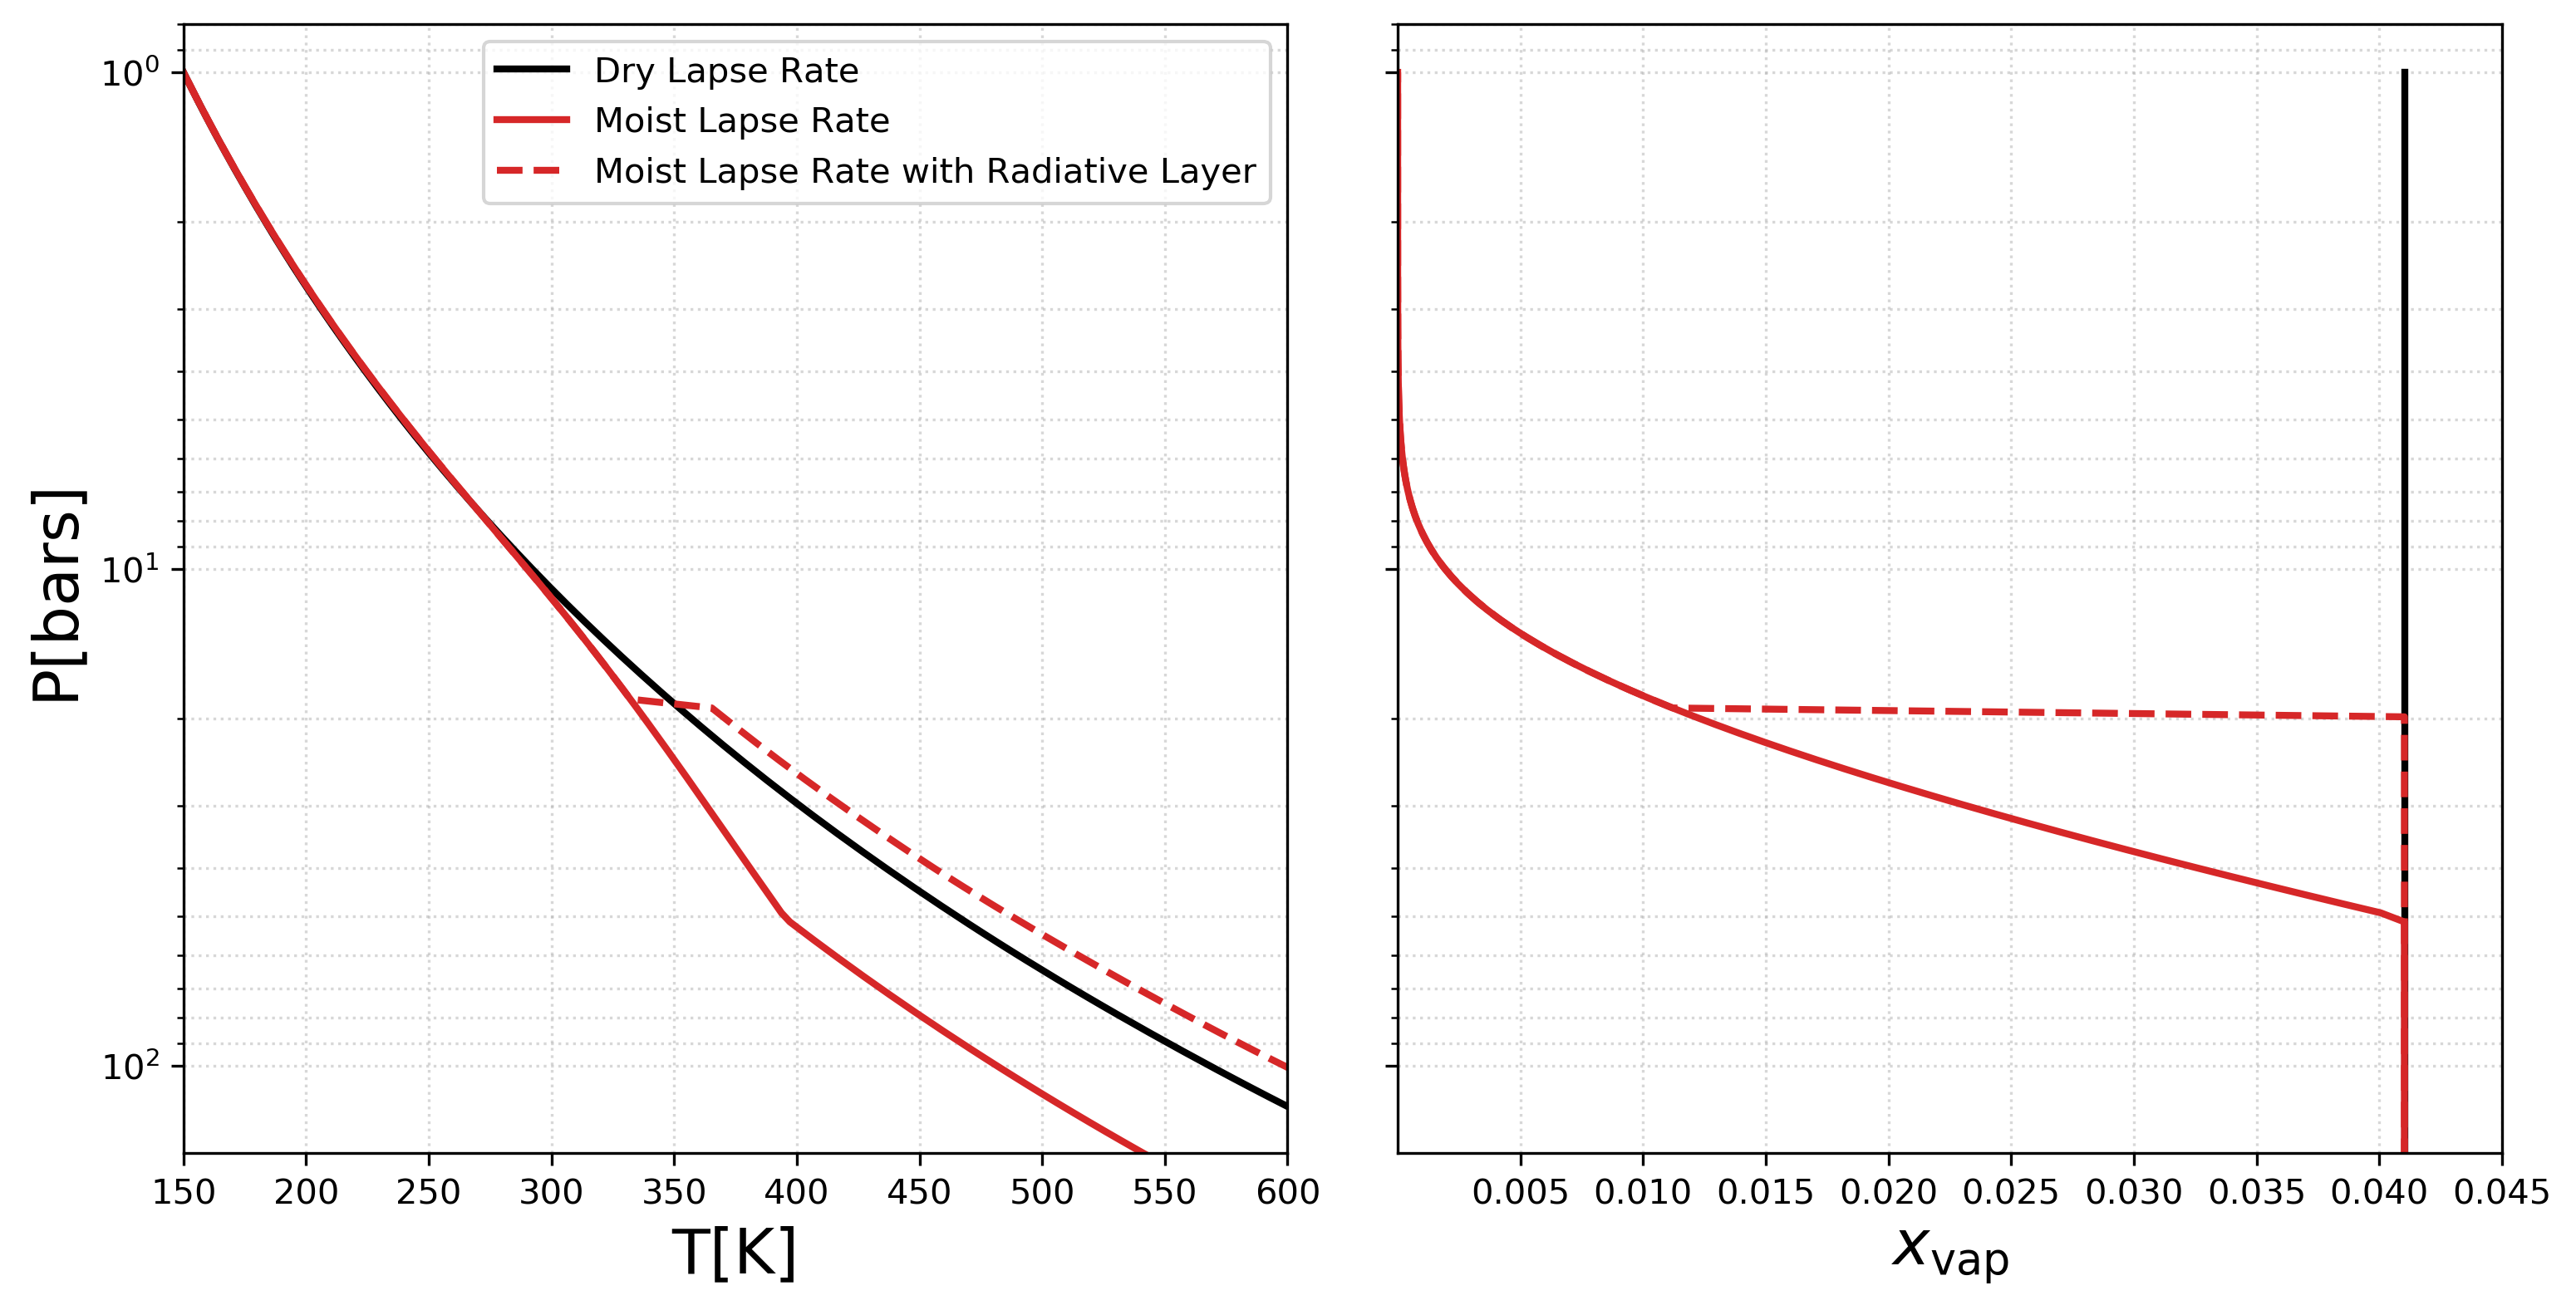
\includegraphics[width=\columnwidth]{figures/comparison_dry_vs_moist_lapse_rates.png}
 }
\caption[A Standard Interior Structure Model]
{Comparison of thermal profiles. The panel on the left is a plot of pressure as a function of temperature. The panel on the right is a plot of pressure as a function of the vapor mole fraction. The solid red line is the pressure profile following moist adiabatic lapse rate. The solid black line is the pressure profile following the the dry adiabatic lapse rate. The dashed red line is the pressure profile following a moist adiabatic lapse rate with the inclusion of a stable radiative layer.} 
\label{fig:comparison_adiabatic_profiles}
\end{figure}
In this figure, we compare profiles that follow a dry adiabat, a moist adiabat, and a moist adiabat containing a stable, radiative layer at some depth. The profile of the moist adiabat is cooler at depth than either of the other two profiles. However, the presence of a stable radiative layer results in a warmer interior. These profiles assume $q_{\rm deep} = 0.25$ and $T_{1} = 150\rm K$, which is approximately when convection is first interrupted in our model Uranus's cooling history, as will be shown in Chapter 3. It is clear from the right-hand panel that when the pressure-temperature profile follows a dry adiabat, the vapor mole fraction, $x_{\rm vap}$, is constant.

To determine when convection is interrupted, we rely on the parameter $\alpha$ \citep{friedson_2017}, which is related to the Ledoux criterion, Equation \ref{eq:ledoux}. $\alpha$ is given by
\begin{equation}
  \alpha = 1 + \xi (q_{\rm s} L / R_{\rm vap} T) ,
  \label{eq:alpha}
\end{equation}
where $R_{\rm vap}$ is the gas constant for the vapor (water), $L$ is the latent heat of vaporization for water, $q_{\rm s}$ is the saturation specific humidity. $q_{\rm s}$ is another way of expressing $x_{\rm vap}^{\rm sat}$. $x_{\rm vap}^{\rm sat}$ is a mass fraction; whereas, $q_{\rm s}$ is a mole fraction. $\xi$ is given by $\xi = \frac{1}{\epsilon} - 1$, where $\epsilon$ is the ratio of the molecular weight of vapor to the mean molecular weight of dry atmosphere. In our case, $\xi \approx -0.872$. When $\alpha$ is negative, the vertical gradient in molecular weight results in a downward stabilizing effect, overwhelming the positive buoyancy effects due to both latent heat release and the density gradient of the surroundings.

\subsubsection{Temperature Jump Across the Water Condensation Zone}
In a layer in which alpha (Eqn.~\ref{eq:alpha}) becomes negative, convection is interrupted. Additionally, in the limit that H$_{2}$O rains out quickly, \citep{friedson_2017,leconte_2017} were able to show that a stable condensation zone can form and that radiative diffusion would be responsible for heat transport within the zone. The temperature gradient across the zone follows a radiative temperature gradient \citep{kippenhahn_2012} given by
\begin{align}
 \nabla_{\rm rad}= \frac{3}{16}\frac{\kappa_{\rm R} P}{g}\frac{T_{\rm int}^4}{T^4} ,
  \label{eq:radiative_gradient}
\end{align}
where $\kappa_{\rm R}$ is the Rosseland mean opacity. We compute $\kappa_{\rm R}$ as follows \citep{2013ApJ...775...10V}:
\begin{equation}
  \kappa_{\rm R} = \kappa_{\rm lowP} + \kappa_{highP},
  \label{eq:kappa1}
\end{equation}
where
\begin{equation}
  \log_{10}\kappa_{\rm lowP} = c_{1}(\log_{10}T - c_{2}\log_{10}P - c_{3})^{2},
  \label{eq:kappalow}
\end{equation}
and 
\begin{equation}
\begin{aligned}
  \log_{10}\kappa_{\rm highP} = & (c_{6} + c_{7}\log_{10}T + c_{8}\log_{10}T^2)  \\ 
                                & + \log_{10}P(c_{9} + c_{10}\log_{10}T) \\ 
                                & + Mc_{11}\bigg(\frac{1}{2} + \frac{1}{\pi}\arctan\bigg({\frac{\log_{10}T - 2.5}{0.2}}\bigg)\bigg),
  \label{eq:kappahigh}
\end{aligned}
\end{equation}
where $M$ is the the metalicity with respect to solar in the logarithmic scale. The values of the coefficients are in Table. \ref{tab:kappa_tab}
\begin{table}[h]
\centering
\begin{tabular}{ccccc}
\multicolumn{1}{l}{}          & \multicolumn{1}{l}{All $T$}    & \multicolumn{1}{l}{}          & \multicolumn{1}{l}{$T < 800$ K} & \multicolumn{1}{l}{$T > 800$ K} \\ \hline
\multicolumn{1}{|c|}{$c_{1}$} & \multicolumn{1}{c|}{$-37.50$}  & \multicolumn{1}{c|}{$c_{6}$}  & \multicolumn{1}{c|}{$-14.051$}  & \multicolumn{1}{c|}{$82.241$}   \\ \hline
\multicolumn{1}{|c|}{$c_{2}$} & \multicolumn{1}{c|}{$0.00105$} & \multicolumn{1}{c|}{$c_{7}$}  & \multicolumn{1}{c|}{$3.055$}    & \multicolumn{1}{c|}{$-55.456$}  \\ \hline
\multicolumn{1}{|c|}{$c_{3}$} & \multicolumn{1}{c|}{$3.2610$}  & \multicolumn{1}{c|}{$c_{8}$}  & \multicolumn{1}{c|}{$0.024$}    & \multicolumn{1}{c|}{$8.754$}    \\ \hline
\multicolumn{1}{|c|}{$c_{4}$} & \multicolumn{1}{c|}{$0.84315$} & \multicolumn{1}{c|}{$c_{9}$}  & \multicolumn{1}{c|}{$1.877$}    & \multicolumn{1}{c|}{$0.7048$}   \\ \hline
\multicolumn{1}{|c|}{$c_{5}$} & \multicolumn{1}{c|}{$-2.339$}  & \multicolumn{1}{c|}{$c_{10}$} & \multicolumn{1}{c|}{$-0.445$}   & \multicolumn{1}{c|}{$-0.0414$}  \\ \hline
\multicolumn{1}{|c|}{}        & \multicolumn{1}{c|}{}          & \multicolumn{1}{c|}{$c_{11}$} & \multicolumn{1}{c|}{$0.8321$}   & \multicolumn{1}{c|}{$0.8321$}   \\ \hline
\end{tabular}
\caption{Coefficients for Equations \ref{eq:kappalow} and \ref{eq:kappahigh}. Table adapted from \citep{2013ApJ...775...10V}}
\label{tab:kappa_tab}
\end{table}

Due to the large opacities that are typical of giant planet interiors, the radiative gradient is significantly larger than either the dry or moist adiabatic gradients. As a result of this steep temperature gradient, the characteristic length (or pressure) scale of the temperature increase is significantly smaller than the radial (or pressure) spacing of our model grid. Instead, the model treats the thin, stable, radiative layer as a discontinuous increase in temperature. Nevertheless, this radiative layer corresponds to a continuum of temperatures that is governed by
\begin{equation}
  T(P) = T_{\rm top} + \int_{P_{\rm top}}^{P_{\rm base}} \left(\frac{dT}{dP}\right)_{\rm rad}\,d P ,
  \label{eq:temp_integral_over_radiative_layer}
\end{equation}
with $P_{\rm top}$ and $T_{\rm top}$ denoting the pressure and temperature at the top of the stable radiative layer, and $P_{\rm base}$ representing the bottom of the layer. The radiative temperature gradient across the radiative layer is nearly constant, so that Eqn.~\ref{eq:temp_integral_over_radiative_layer} simplifies to
\begin{align}
T_{\rm base}\equiv T(P+\Delta P) &= T_{\rm top} + \left(\frac{dT}{dP}\right)_{\rm rad}\Delta P ,
\label{eq:temperature_profile_over_radiative_layer_simplification}
\end{align}
where $\Delta P$ is the extent of the pressure-space of the radiative layer, given by
\begin{align}
\Delta P \equiv P_{\rm base}-P_{\rm top} &= \frac{P_{\rm sat}(T_{\rm base})}{x_{\rm vap}^{\rm deep}} - P_{\rm top}.
\label{eq:delta_P_over_radiative_layer}
\end{align}
As in the rest of the outer envelope, we suppose that saturation holds in the radiative layer so that the vapor mole fraction, $x_{\rm vap}$, is equal to the saturated vapor mole fraction:
\begin{align}
x_{\rm vap}(P, T) &= x_{\rm vap}^{\rm sat}(P, T) = \frac{P_{\rm sat}(T)}{P}, \qquad P<P_{\rm base}.
\label{eq:vapor_mole_fraction_within_condensation_zone}
\end{align}
The base of the stable radiative layer is set by the condition that $x_{\rm vap}$ has reached the deep water value $x_{\rm vap}^{\rm deep}$:
\begin{align}
x_{\rm vap}^{\rm sat}(P_{\rm base}, T_{\rm base}) &= \frac{P_{\rm sat}(T_{\rm base})}{P_{\rm base}}=x_{\rm vap}^{\rm deep},
\label{eq:cloud_base}
\end{align}
and at deeper levels, the region is subsaturated and hence no condensation occurs. Temperatures below the stable radiative layer are obtained by integrating the dry adiabat $\nabla_{\rm ad}$:
\begin{align}
T(P) &= T_{\rm base} + \int_{P_{\rm base}}^P\left(\frac{dT}{dP}\right)_{\rm ad}\,d P, \qquad  P>P_{\rm base} .
\label{eq:dry_adiabat_integration}
\end{align}


\chapter{Results}

\section{Condensation-inhibited Convection}
In Figure~\ref{fig:convection_inhibited}, we show the results of our initial exploratory models. We show $\alpha$ with respect to $P$, $x_{\rm vap}$, and $T$. 
\begin{figure}[h]{}
 \centerline{
  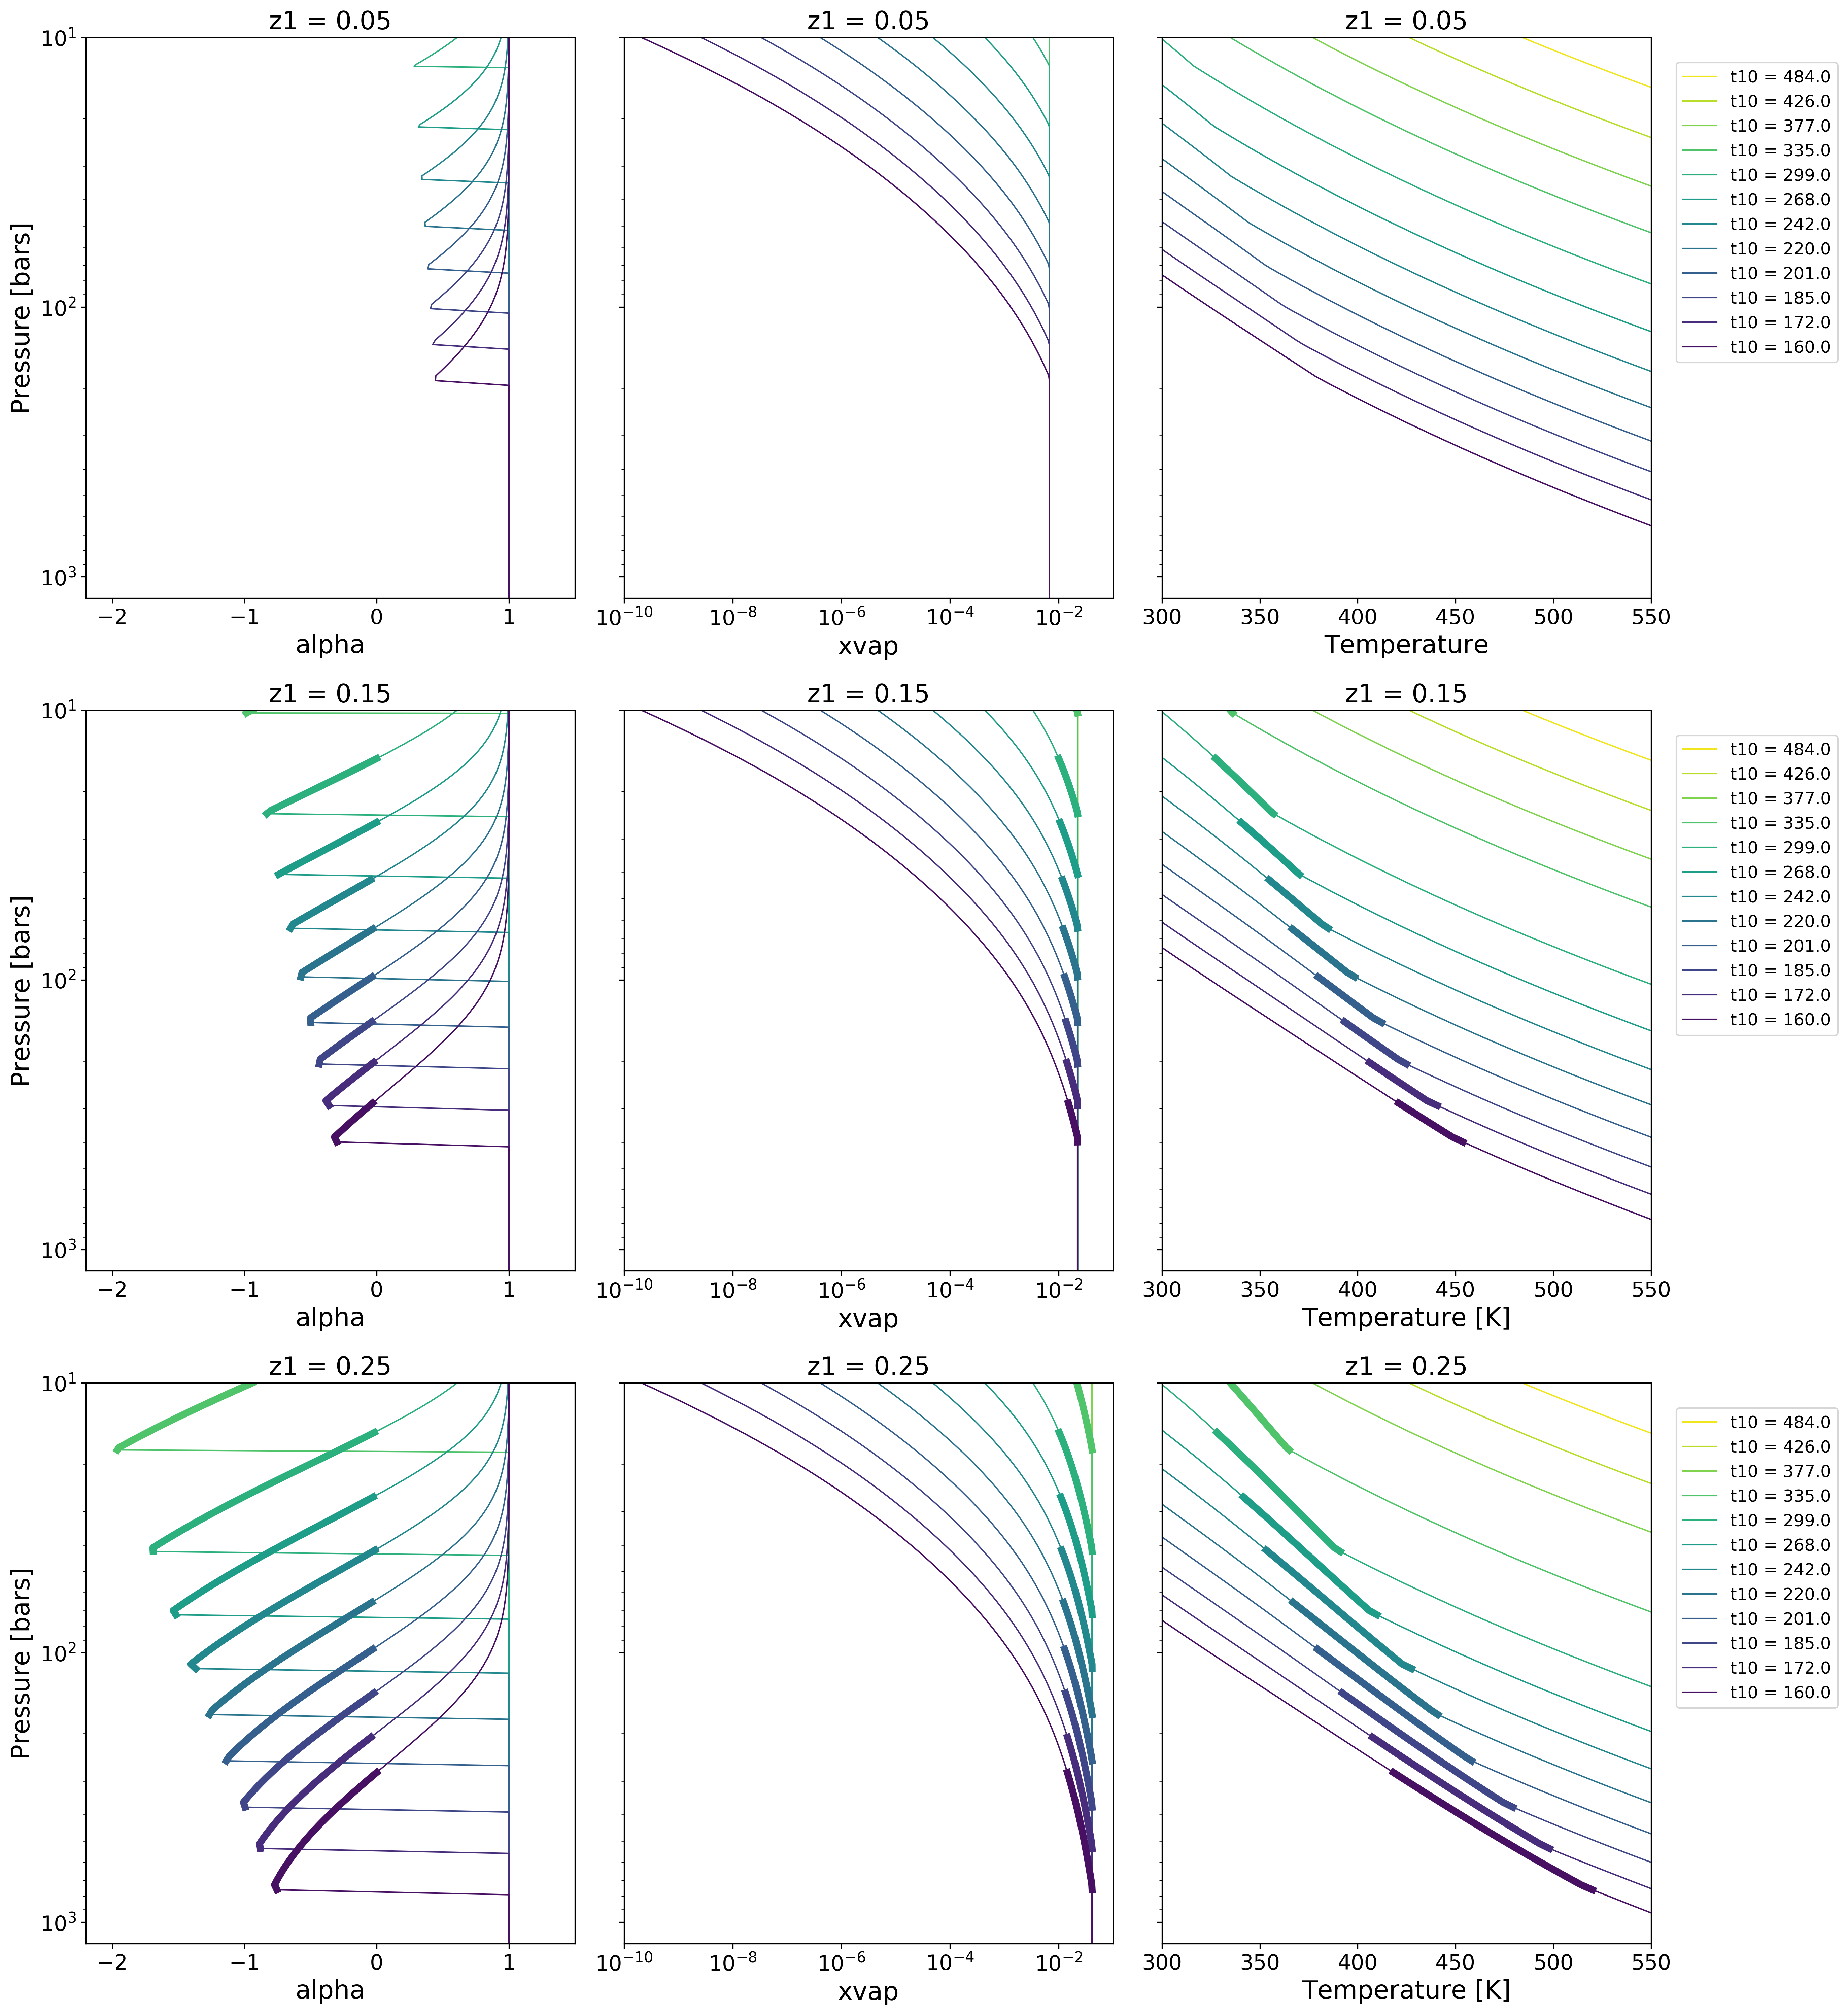
\includegraphics[width=\columnwidth]{figures/convection_inhibited_2.png}
 }
\caption[Inhibition of convection on Uranus]
{Moist adiabatic profiles for Uranus as a function of  $q_{\rm deep}$. Each plot is an evolutionary sequence from hot/early (yellow) to cool/late (purple). Each row represents a different value for $q_{\rm deep}$. For $q_{\rm deep} = 0.05$, no stable condensation zone forms. For $q_{\rm deep} = 0.15$ and $q_{\rm deep} = 0.25$, convection is inhibited by condensation. The shaded regions indicate where $\alpha$ is negative.}
\label{fig:convection_inhibited}
\end{figure}
These static models are run for a variety of $T_{10}$, the planet's temperature at $P=10$ bars. Larger $T_{10}$ represents warmer episodes in the planet's past, while smaller $T_{10}$ represents cooler, more recent episodes in the planet's history.  It is important to highlight that the bulk water abundance for Uranus and Neptune is unconstrained \citep{guillot_1995}. Therefore, these model runs use three different values of $q_{\rm deep}$, searching for deep water abundances and evolutionary phases for which convection is inhibited by water condensation. In these exploratory models, we only consider the model Uranus. We find that for $q_{\rm deep} = 0.05$, convection is not interrupted. In other words, $\alpha$ (Eqn.~\ref{eq:alpha})  never takes on negative values with this concentration of water vapor, hence the condition for stability is never met. However, for larger values of $q_{\rm deep}$, we find that $\alpha$ does take{} on negative values (see rows 2 and 3 in Figure ~\ref{fig:convection_inhibited}). These findings are in agreement with \citep{friedson_2017,leconte_2017} who both found a critical water abundance, $q_{\rm deep}$, of approximately $8\%$. The shaded regions of the plots indicate the pressure-space over which $\alpha$ is negative. It is important to note that with these exploratory models, we neglect the stable radiative layer's impact on the interior's thermal structure. More specifically, these profiles describe a scenario in which moist convection occurs throughout. As such, the shaded regions appear extended, when in reality the top of the shaded region indicates where the top of the stable radiative layer would form. As we will see in Section 2.3, self-consistent models that account for the formation of a stable layer, with a critical $q_{\rm deep}$, will show pressure-temperature profiles with an abrupt temperature increase at the location of the radiative layer. Looking at the plots for $q_{\rm deep} = 0.15$ and $q_{\rm deep} = 0.25$, we can see that convection is interrupted roughly when $T_{10} = 335$ K. With regard to the vapor mole fraction panels on the right of Figure~\ref{fig:convection_inhibited}, we can see that for a hot model Uranus, $x_{\rm vap}$ profiles are vertical, taking on a constant value as expected. For cooler Uranus models, we see that as water condenses out, $x_{\rm vap}$ decreases. In the temperature-pressure profiles, we can see a kink in the graphs, corresponding to $x_{\rm vap}$ taking on a constant value. In other words, the region has become sub-saturated and from that point, the profile follows a dry adiabat. Finally, we can see that as the planet cools, the condensation zones descend deeper into the interior.




\section{Formation of Radiative Layer}
Now we turn our focus to static models, again using only our model Uranus, that explicitly allow for the formation of stable radiative layers when conditions are suitable, as determined by the stability criterion, $\alpha$ (Eqn.~\ref{eq:alpha}). The plots in Figure~\ref{fig:radiative} show the temperature profile and vapor mole fraction for H$_{2}$O for three different values of $q_{\rm deep}$: $0.05$, $0.15$, and $0.25$. 
\begin{figure}[ht]
 \centerline{
  \includegraphics[width=\columnwidth]{figures/uranus_thesis_static_radiative_layer_plots_without_grid_points_more_qdeeps.png}
 }{}
\caption[Formation of Radiative Layer]
{Moist adiabatic profiles that allow for formation of stable water condensation zones. From top to bottom, we move from $q_{\rm deep} = 0.05$, $0.15$, and $0.25$, respectively. $T_{10}$ varies from hotter (yellow) to cooler (purple), more recent temperatures.}
\label{fig:radiative}
\end{figure}
In the top row, we can see that for early $T_{10}$'s, there is no onset of condensation, and the warmer profiles follow a dry adiabat. For later, cooler $T_{10}$'s, there is a visible kink in the lapse rate which indicates the onset of condensation, at which point the lapse rate has a shallower slope. For the larger values of $q_{\rm deep}$, where $\alpha$ takes on negative values, we see the onset of condensation-inhibited convection and the formation of a stable radiative layer. The water condensation zones ar{}e represented by the horizontal discontinuities moving from left to right. As the planet cools, these radiative layers descend deeper into the planet's interior. When the radiative layers are established, the interior below the zone becomes much warmer. 

In Figure~\ref{fig:overlay}, we highlight the effect of a warming interior where we have overlaid the profiles for $q_{\rm deep} = 0.25$ (exhibiting stable radiative layers) over the profile for $q_{\rm deep}=0.05$ (no stable layers). 
\begin{figure}[h]{}
 \centerline{
  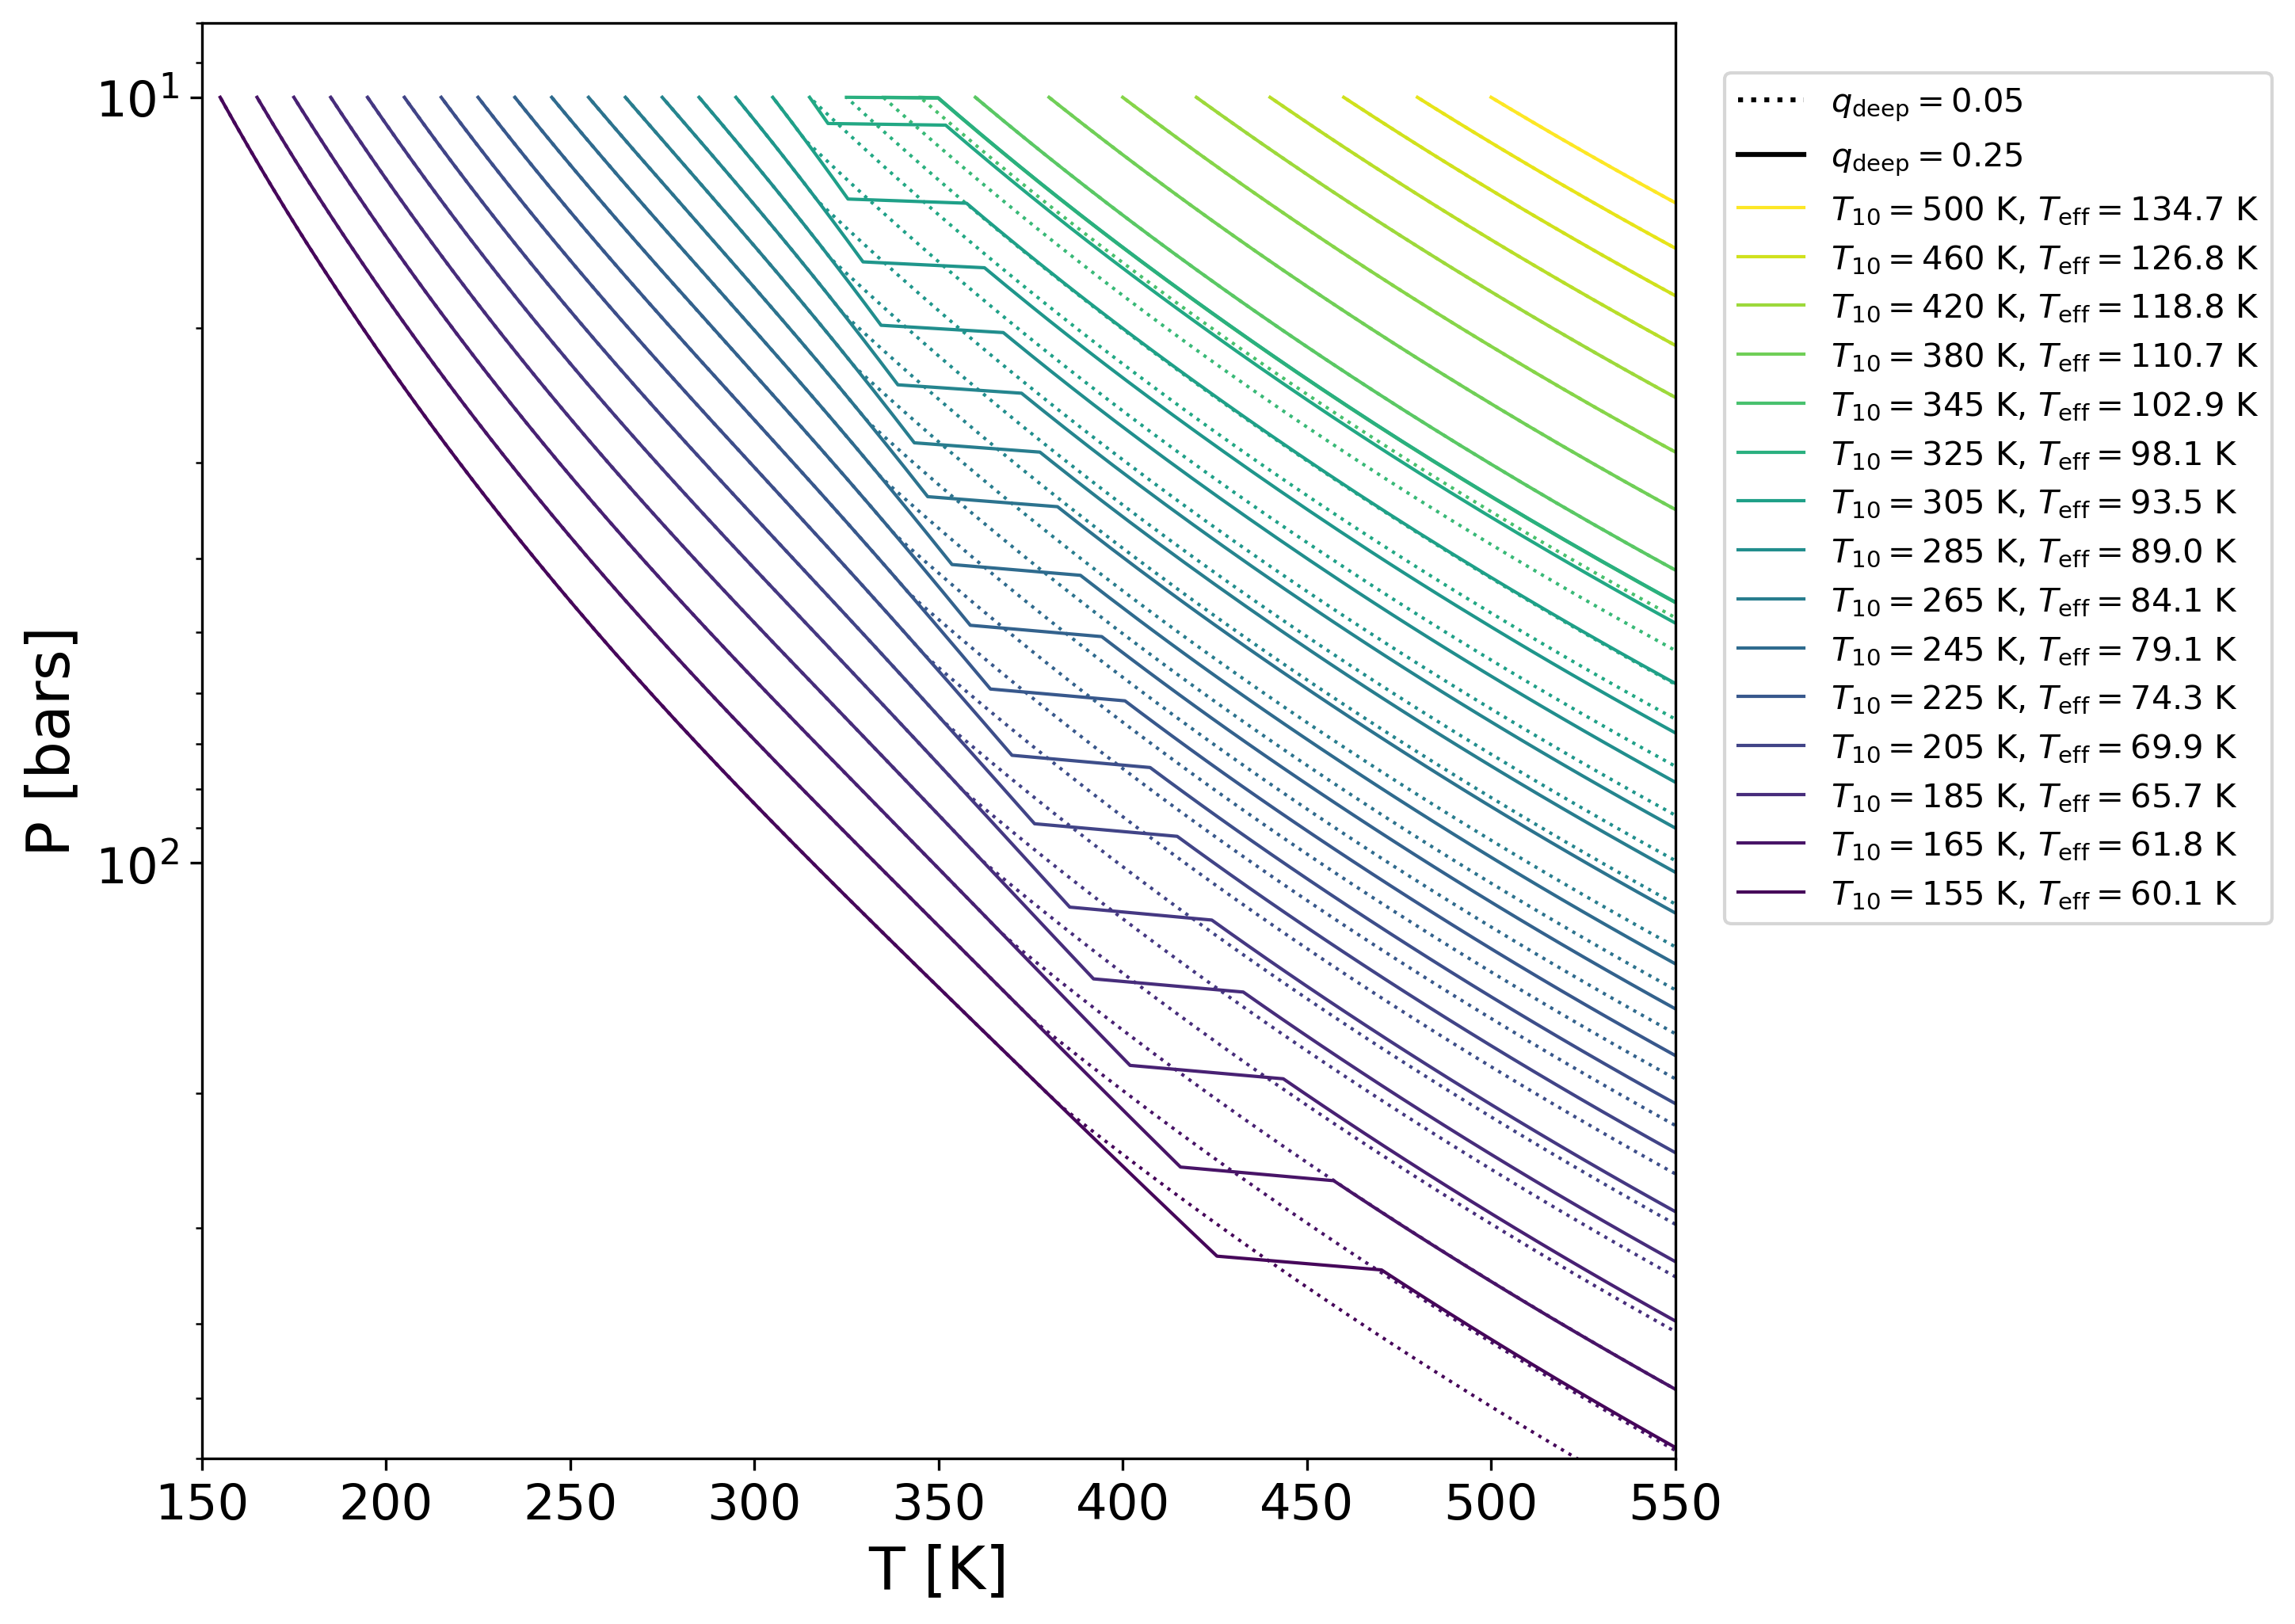
\includegraphics[width=\columnwidth]{figures/thesis_static_radiative_layer_plot_diff_qdeep_overlay.png}
 }
\caption[Impact of Radiative Layer on $T_{10}$]
{Overlay of profiles with different deep water abundances, highlighting impact of stable water condensation zones on a planet's thermal structure. The solid lines represent the pressure-temperature profile for $q_{\rm deep} = 0.25$, and the dashed lines for $q_{\rm deep}=0.05$. Note the effect of the radiative layer in the sequence where $q_{\rm deep} = 0.25$. The temperature jump results in a deep interior that resembles an earlier $T_{10}$, and thus an earlier evolutionary phase for the sub-critical, $q_{\rm deep} = 0.05$, model.}
\label{fig:overlay}
\end{figure}
From this plot, one can see that the presence of a radiative layer creates a temperature jump such that a given $T_{10}$ appears to look like an earlier $T_{10}$. In other words, we find that the steep temperature increase caused by the presence of a radiative layer causes the interior to be much hotter than one would find using a simple moist adiabatic model with no stable layers. So, for a fixed $T_{10}$, while sub-critical ($q_{\rm deep} = 0.05$) and super-critical ($q_{\rm deep} = 0.25$) models may appear identical near the surface, the super-critical model has a much warmer interior, one that resembles an earlier evolutionary phase at a higher $T_{10}$. Looking at the adjacent $x_{\rm vap}$ plots, we can see that $x_{\rm vap}$ follows its saturated value. At the bottom of the radiative layer, the vapor mole fraction equals its deep water value, which is the condition that sets the base of the condensation zone (Eqn. \ref{eq:cloud_base}). 


\section{Thermal Evolution of Uranus and Neptune}

% cooling camparisons of dry adiabat, moist adiabat, and moist adiabat with radiative layer
In Figure~\ref{fig:evolve_adiabats}, we display the results of evolutionary tracks that consider separately the evolution of a dry adiabat, a moist adiabat with condensation but no stable radiative layer, and a moist adiabat with condensation containing stable radiative layers. For all of these evolutionary tracks, we assume $q_{\rm deep} = 0.25$. 
\begin{figure}[h]
 \centerline{
  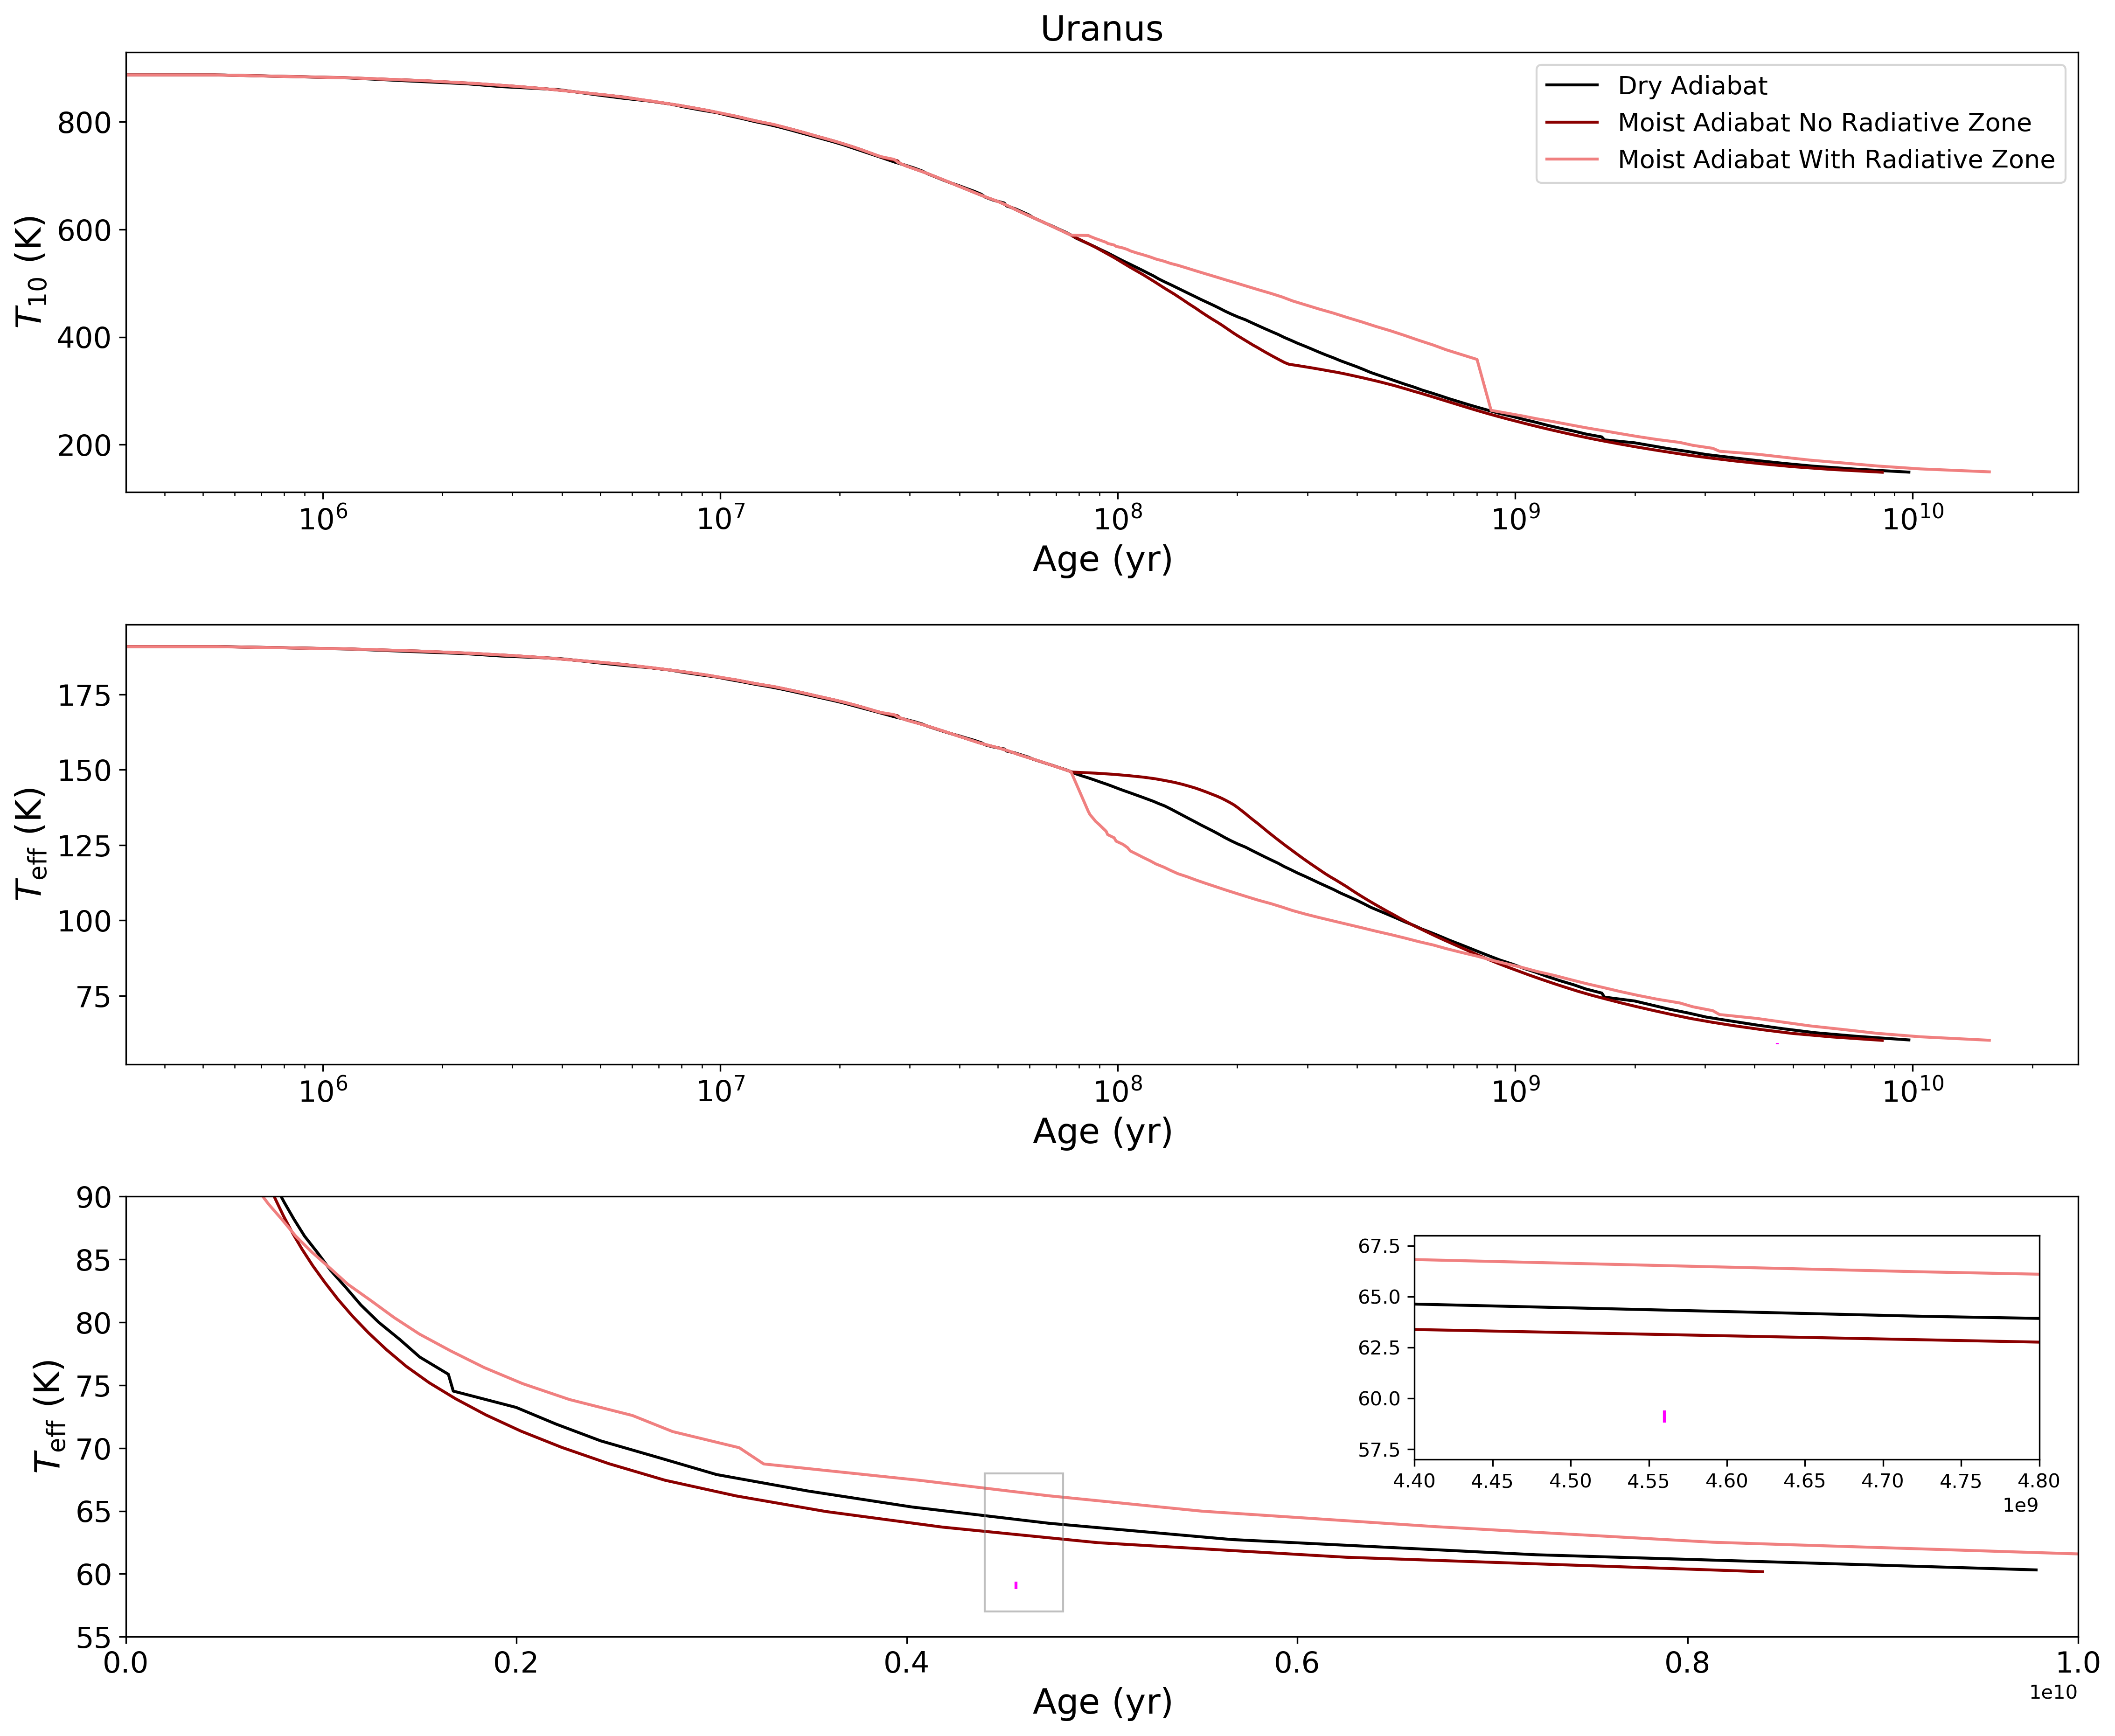
\includegraphics[width=\columnwidth]{figures/dry_moist_radiative_u_cooling_curves_adiabat_comparisons.png}
 }
\caption[Thermal Evolution Curves for Uranus - Adiabat Comparisons]
{Thermal evolution of Uranus comparing the impact of dry convection, moist convection, and moist convection allowing for formation of stable condensation zone. The top panel is a plot of $T_{10}$ over log time. The middle panel is a plot of $T_{\rm eff}$ over log time. The bottom panel is a plot of $T_{\rm eff}$ over linear time. The black line represents the thermal evolution for a dry adiabat. The dark red line represents the thermal evolution for a moist adiabat that does not allow for the formation of a stable radiative layer. The light red line represents the thermal evolution of a moist adiabat that does allow for the formation of a stable radiative layer. The blue vertical line on the lower panel represents the currently observed effective temperature of Uranus with 2$\sigma$ errors for clarity. }
\label{fig:evolve_adiabats}
\end{figure}
The coolest scenario at present time is a moist adiabat that is never stable against convection. The moist adiabat that allows for the formation of stable radiative layers has the warmest outcome at present time. 

In Figure~\ref{fig:evolve_uranus_qdeeps} (Uranus) 
% cooling uranus
\begin{figure}[h]
 \centerline{
  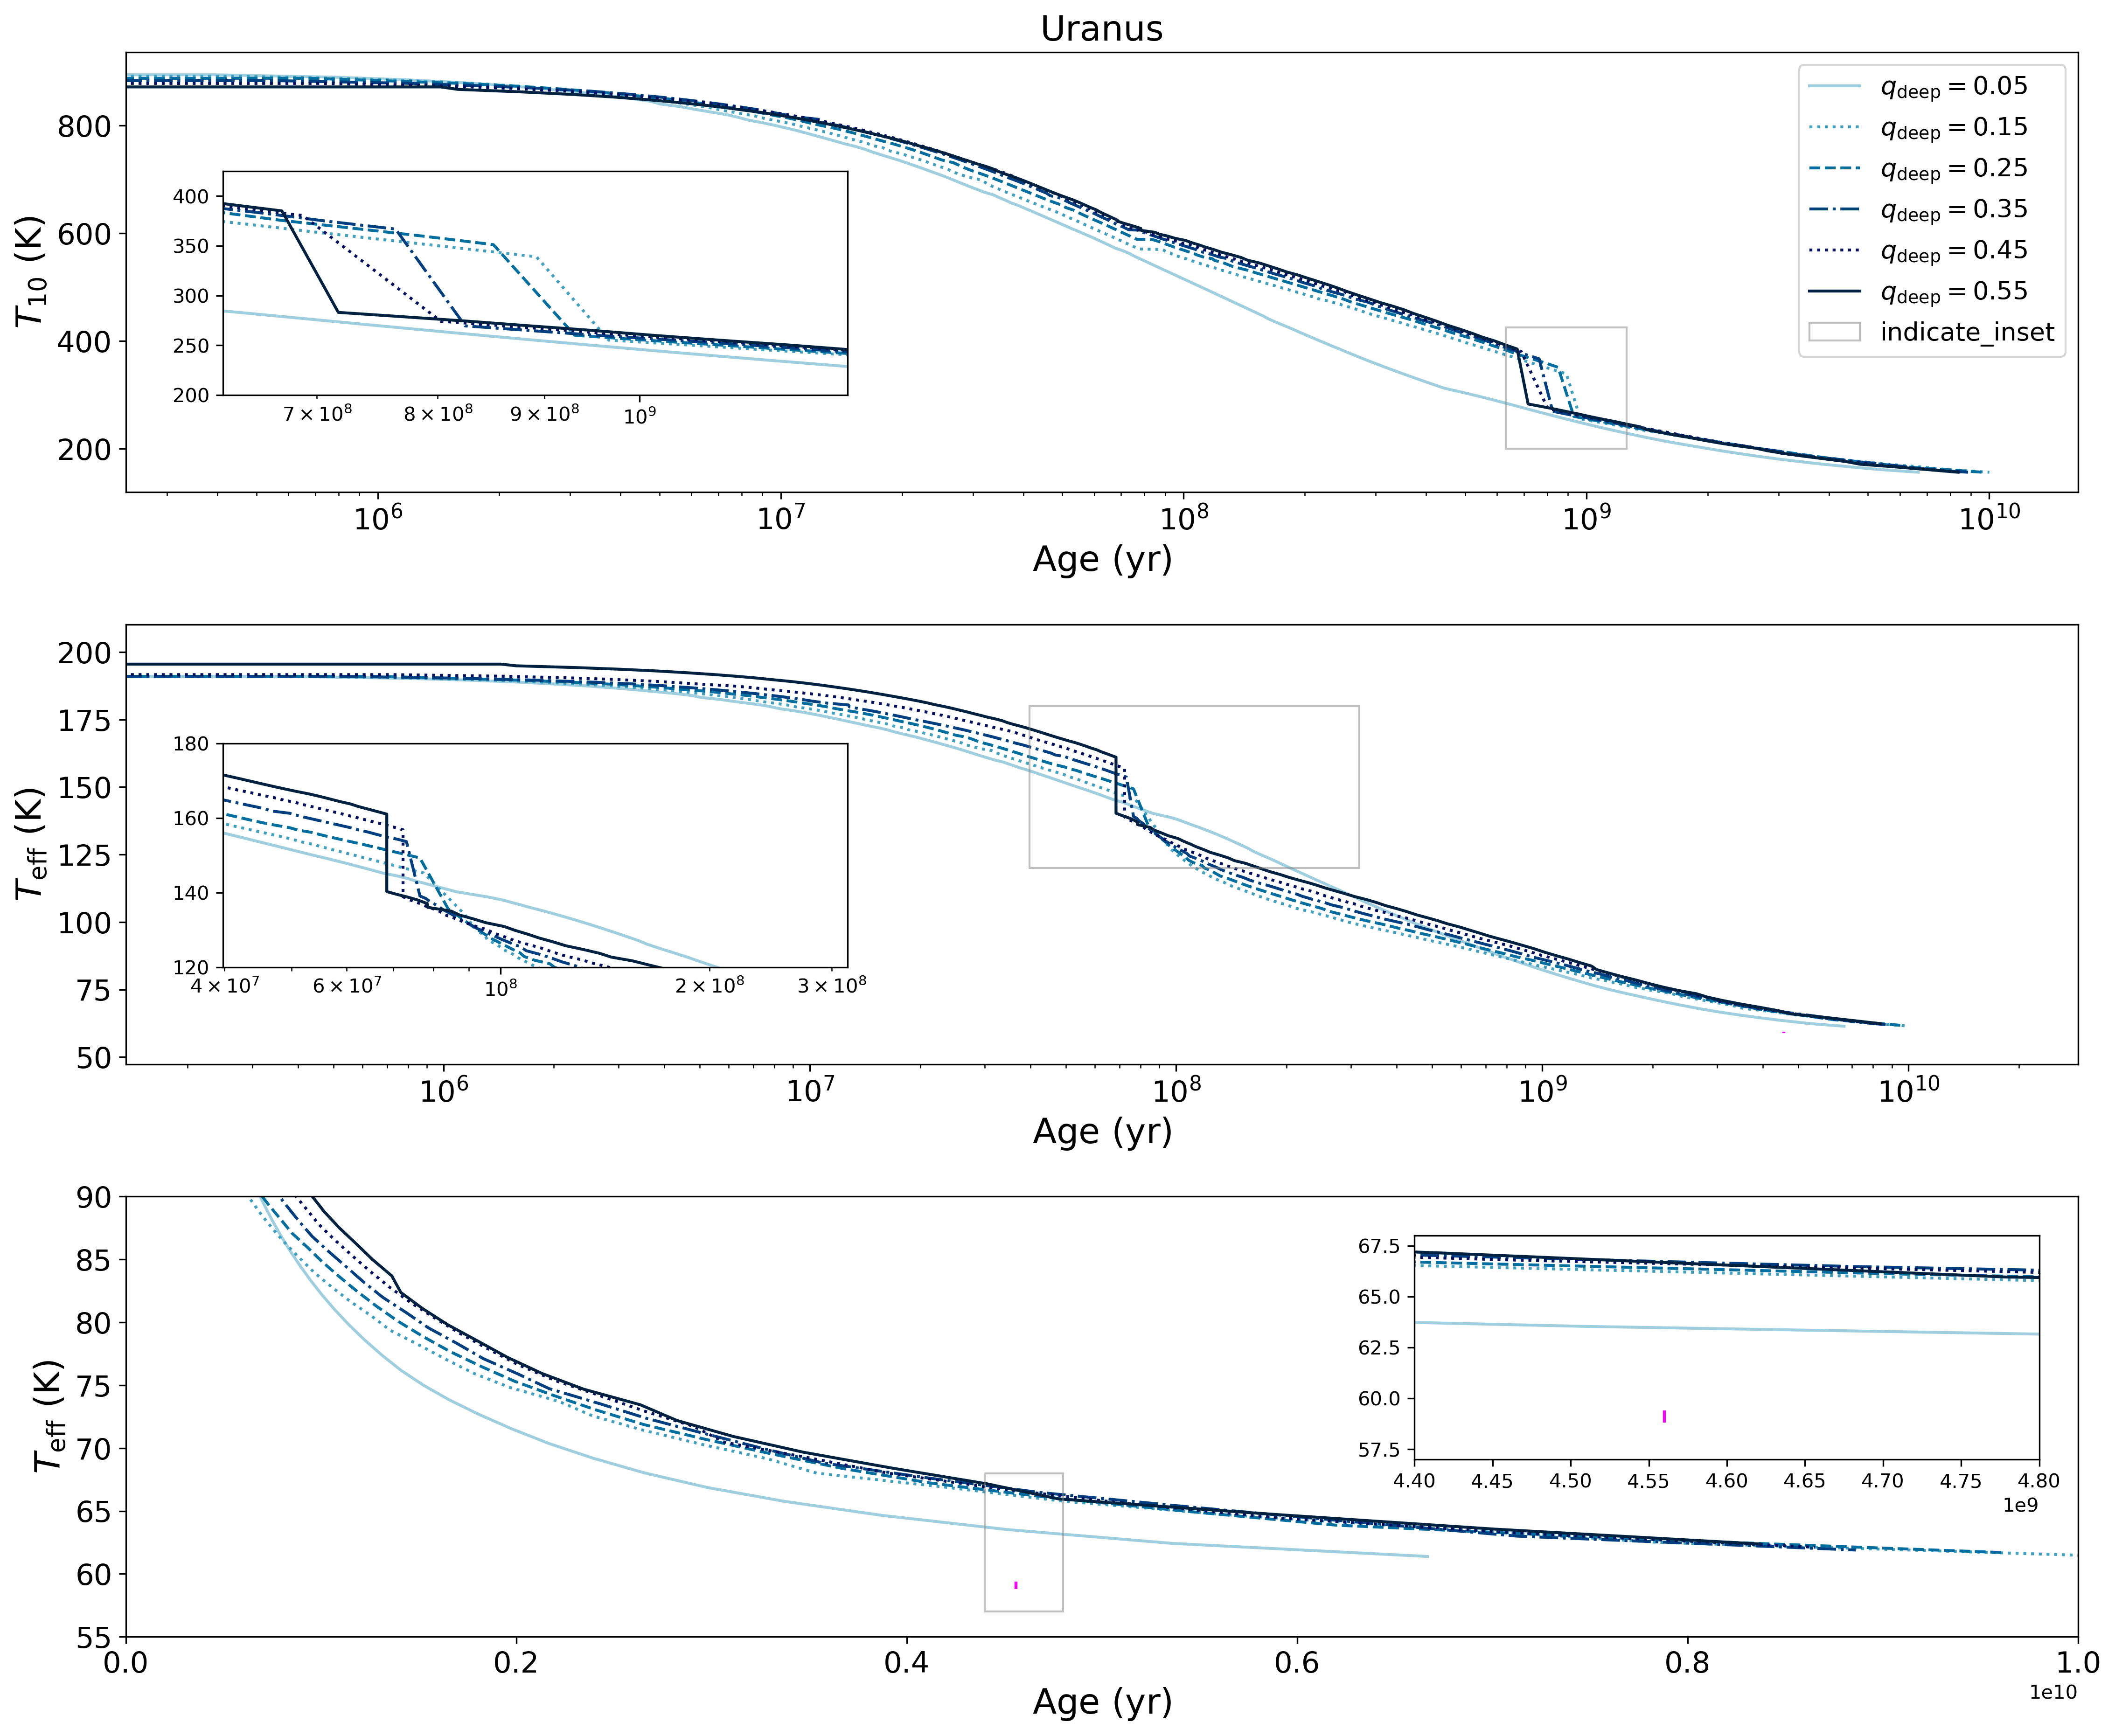
\includegraphics[width=\columnwidth]{figures/u_cooling_curves_nz_4096_more_qdeeps.png}
 }
\caption[Thermal Evolution Curves for Uranus - Water Vapor Concentration Comparisons]
{Thermal evolution of Uranus as a function of deep water abundance. These evolutionary tracks are generated by full models that allow for condensation and the formation of stable radiative layers if conditions are suitable. The curves in these plots represent thermal evolution tracks for different values of $q_{\rm deep}$. Dark blue is the largest concentration of water vapor, at $q_{\rm deep} = 0.55$ and the light blue line is the least concentration of water vapor at $q_{\rm deep} = 0.05$. The insets in the top two panels zoom in on periods of rapid cooling (the initial onset of condensation-inhibited convection). The vertical fuchsia line represents the current $T_{\rm eff}$ with $2\sigma$ errors for clarity.}
\label{fig:evolve_uranus_qdeeps}
\end{figure}
and Figure~\ref{fig:evolve_neptune_qdeeps} (Neptune), we consider the impact of different concentrations of $q_{\rm deep}$ on the thermal evolution of Uranus and Neptune. As the planets cool, their radiative layers descend deeper into the interior, as we saw in Figure~\ref{fig:overlay}. The formation and impact of the radiative layer is also noticeable in the thermal evolution plots. Looking at the $T_{\rm eff}$ panels, the onset of condensation-inhibited convection resulting from the formation of a stable radiative layer is clearly visible, seen as a discontinuous temperature drop at ~$7 \times 10^7$ yr. This rapid cooling event is due to the radiative layer acting as an imperfect thermal insulator, trapping heat below the radiative layer, forcing the interior to cool more slowly. By contrast, the insulating effect of the radiative layer allows the envelope above to cool more rapidly. 

Similarly, ~$7 \times 10^8$ yr, in the $T_{10}$ panels for Figures \ref{fig:evolve_uranus_qdeeps} and \ref{fig:evolve_neptune_qdeeps}, we see similar rapid cooling episodes. But, here the radiative layer has descended further, and is now trapping heat even deeper in the interior, while also allowing the envelope above to cool more rapidly.

We also look at the impact of $q_{\rm deep}$ on the evolution of planetary radius in Figure \ref{fig:evolve_uranus_radius} (Uranus) and Figure \ref{fig:evolve_neptune_radius} (Neptune) and find that larger deep water concentrations tend to converge more closely toward the presently observed radius for both Uranus and Neptune in these simulations. It's important to highlight that we could possibly converge toward the currently observed radii for both planets by increasing the $Z_{2}$ mass fraction, or by increasing the core mass for a given $q_{\rm deep}$. In other words, from these model runs it is clear that the deep water concentration ($q_{\rm deep}$) within the outer envelope has an impact on planetary radii; so too could variations in core mass and the water mass fraction within the inner envelope. 
%  cooling neptune
\begin{figure}[h]
 \centerline{
  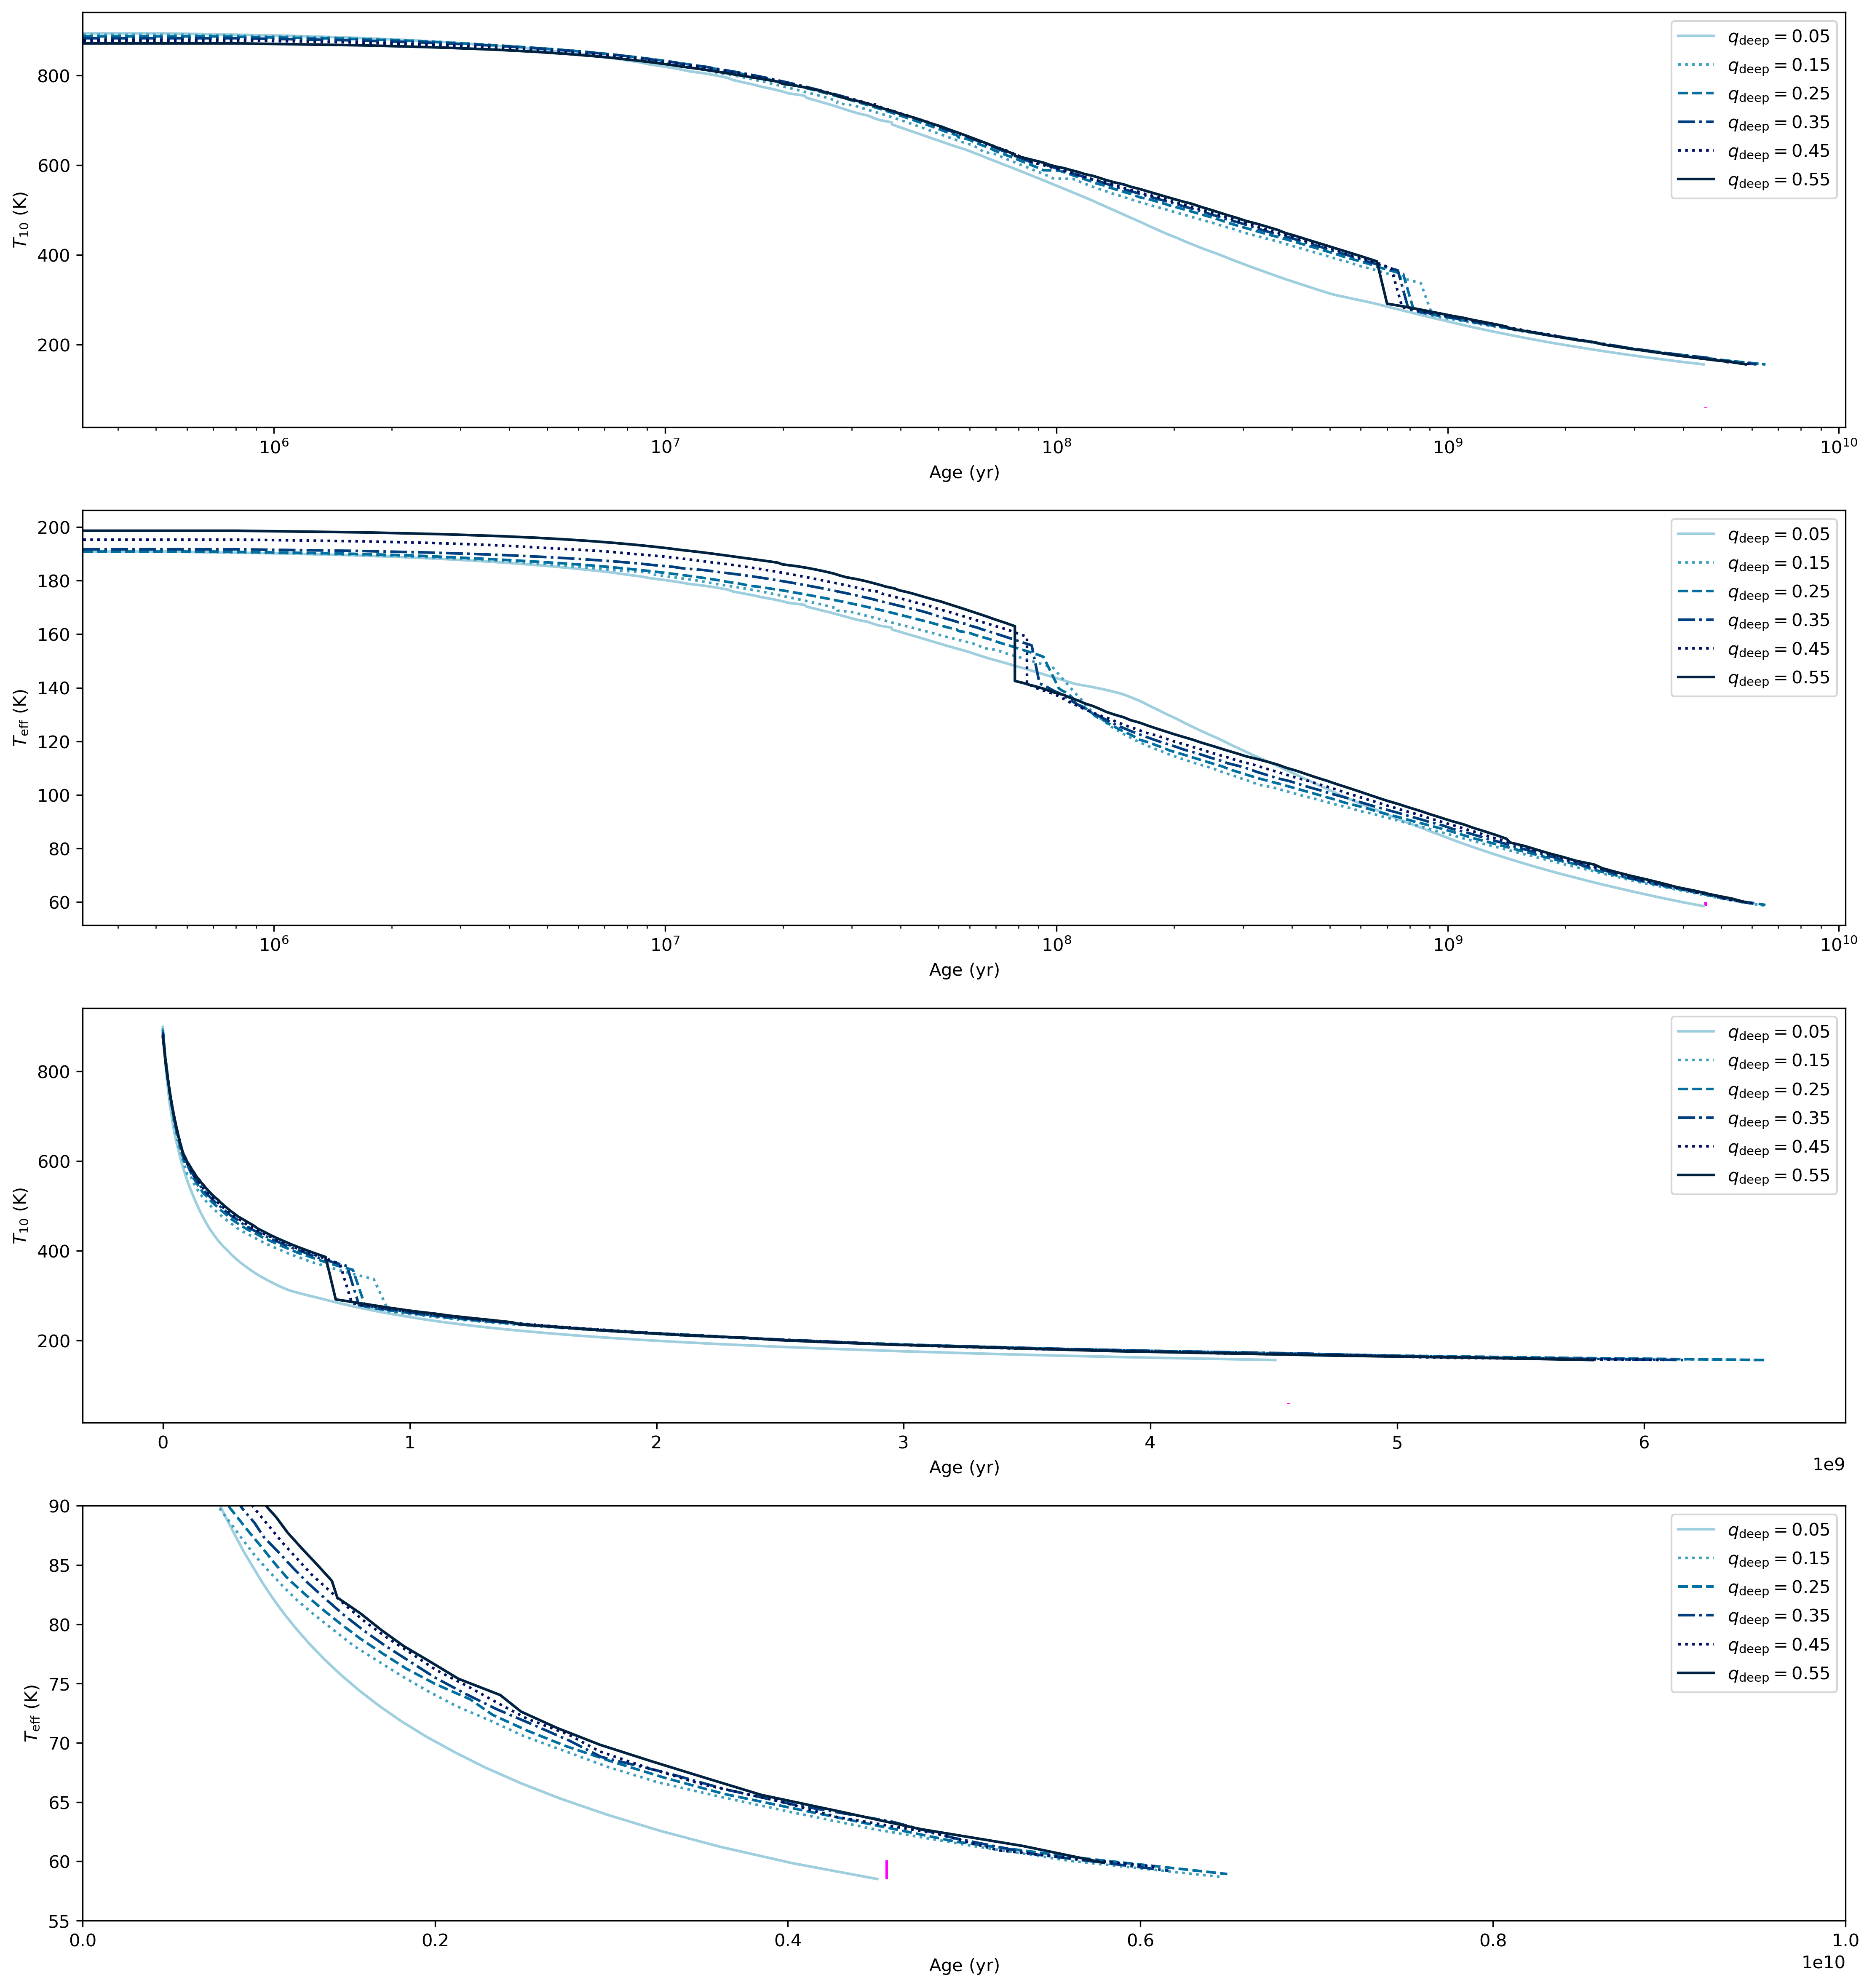
\includegraphics[width=\columnwidth]{figures/n_cooling_curves_nz_4096_more_qdeeps.png}
 }
\caption[Thermal Evolution Curves for Neptune - Water Vapor Concentration Comparisons]
{As in Figure \ref{fig:evolve_uranus_qdeeps}, but for Neptune instead of Uranus.}
\label{fig:evolve_neptune_qdeeps}
\end{figure}
%  cooling radius curves
\begin{figure}[h]
 \centerline{
  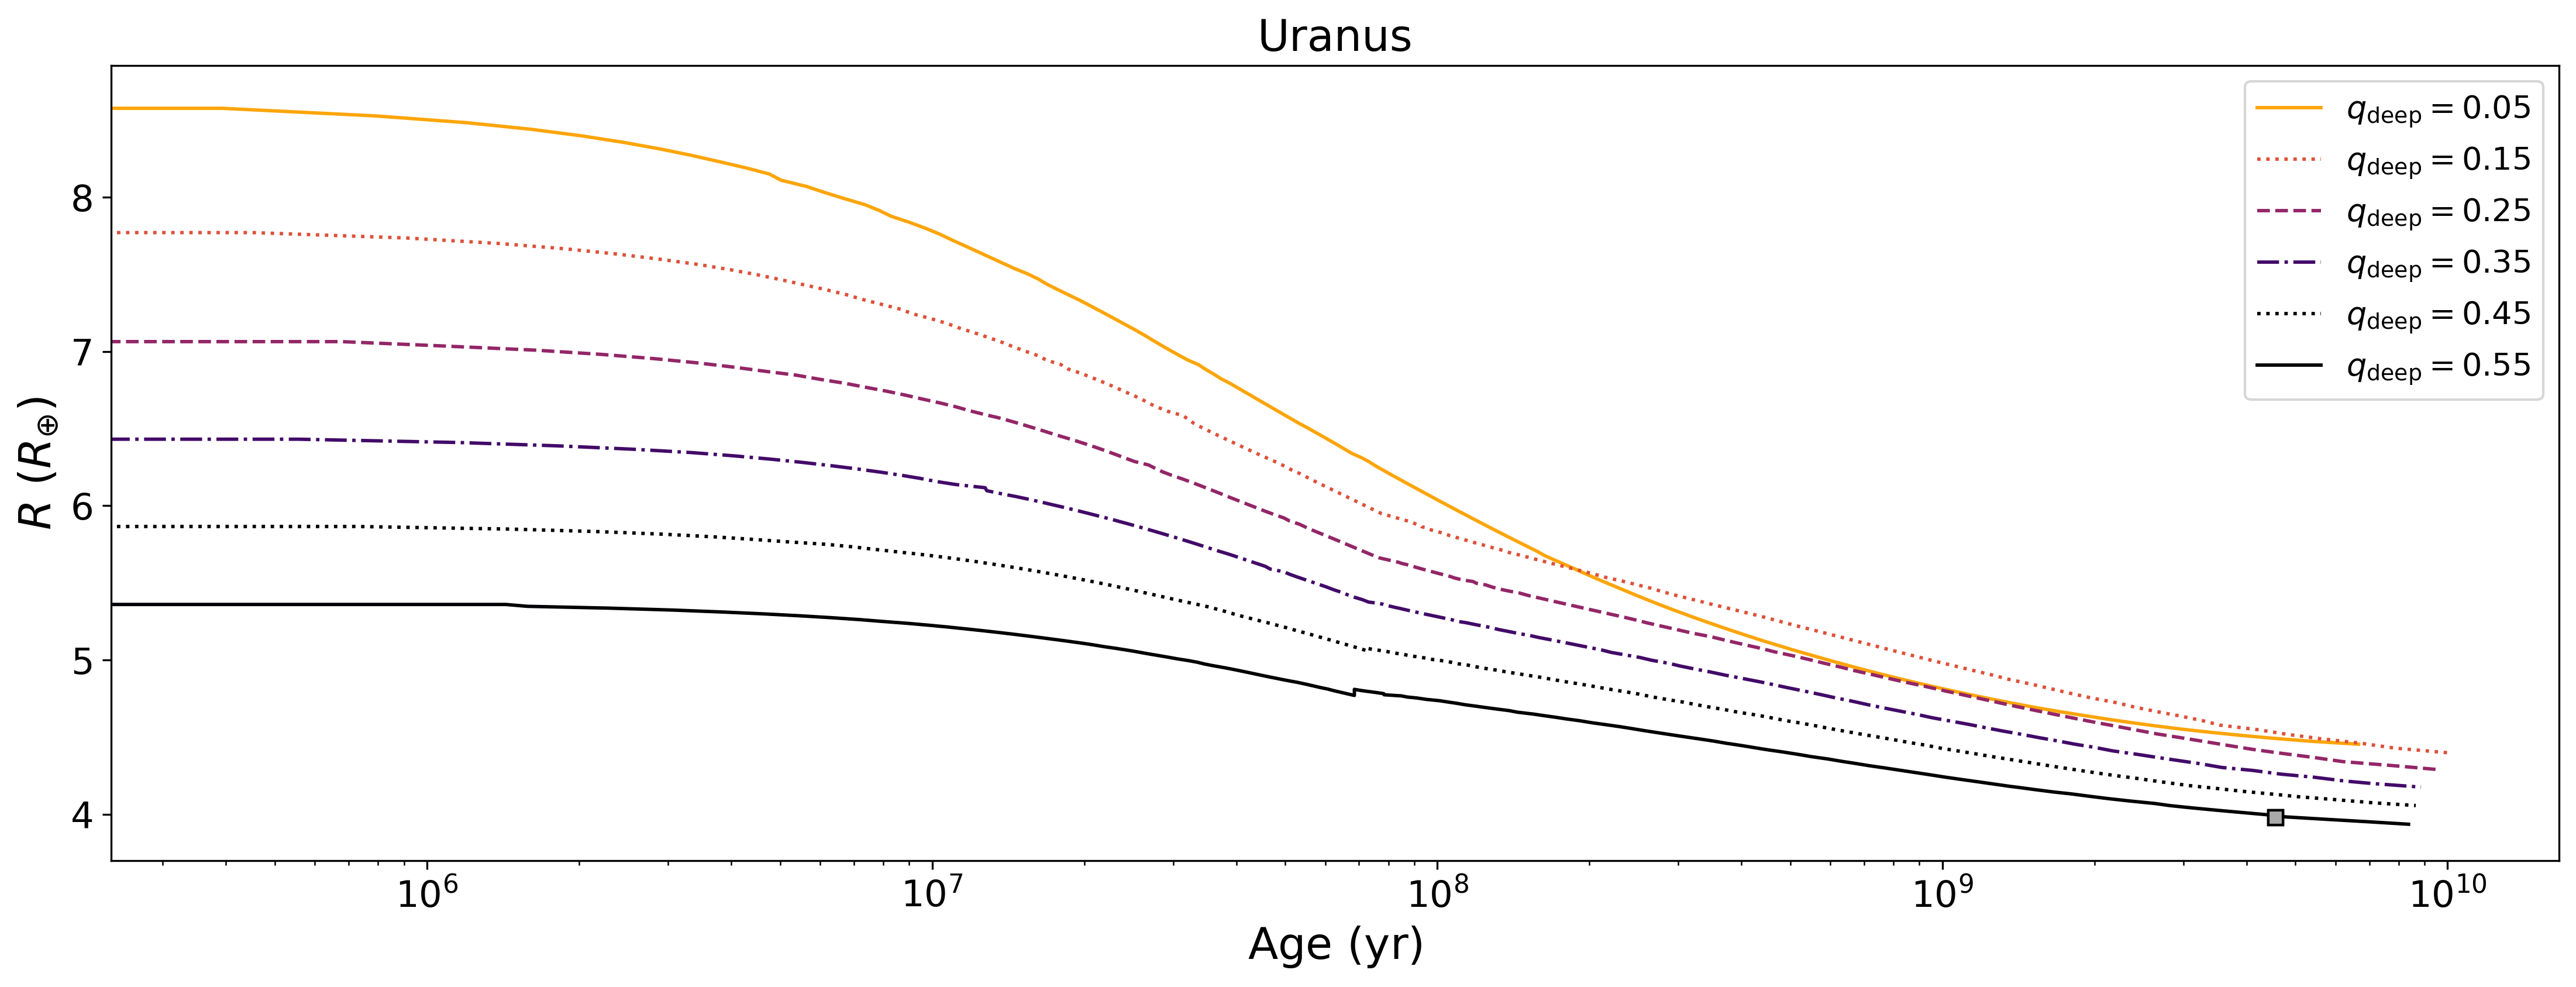
\includegraphics[width=\columnwidth]{figures/u_cooling_radius_nz_4096_logx_more_qdeeps.png}
 }
\caption[Thermal Evolution Curves for Uranus - Radius]
{Evolution of Uranus's radius as a function of deep water abundance. The gray square represents the current observed radius. The different curves (colors / line styles) correspond to different water abundances as labeled in the figure. Larger values of $q_{\rm deep}$ converge more closely on the present observed value of Uranus's radius. }
\label{fig:evolve_uranus_radius}
\end{figure}

 
\begin{figure}[h]
 \centerline{
  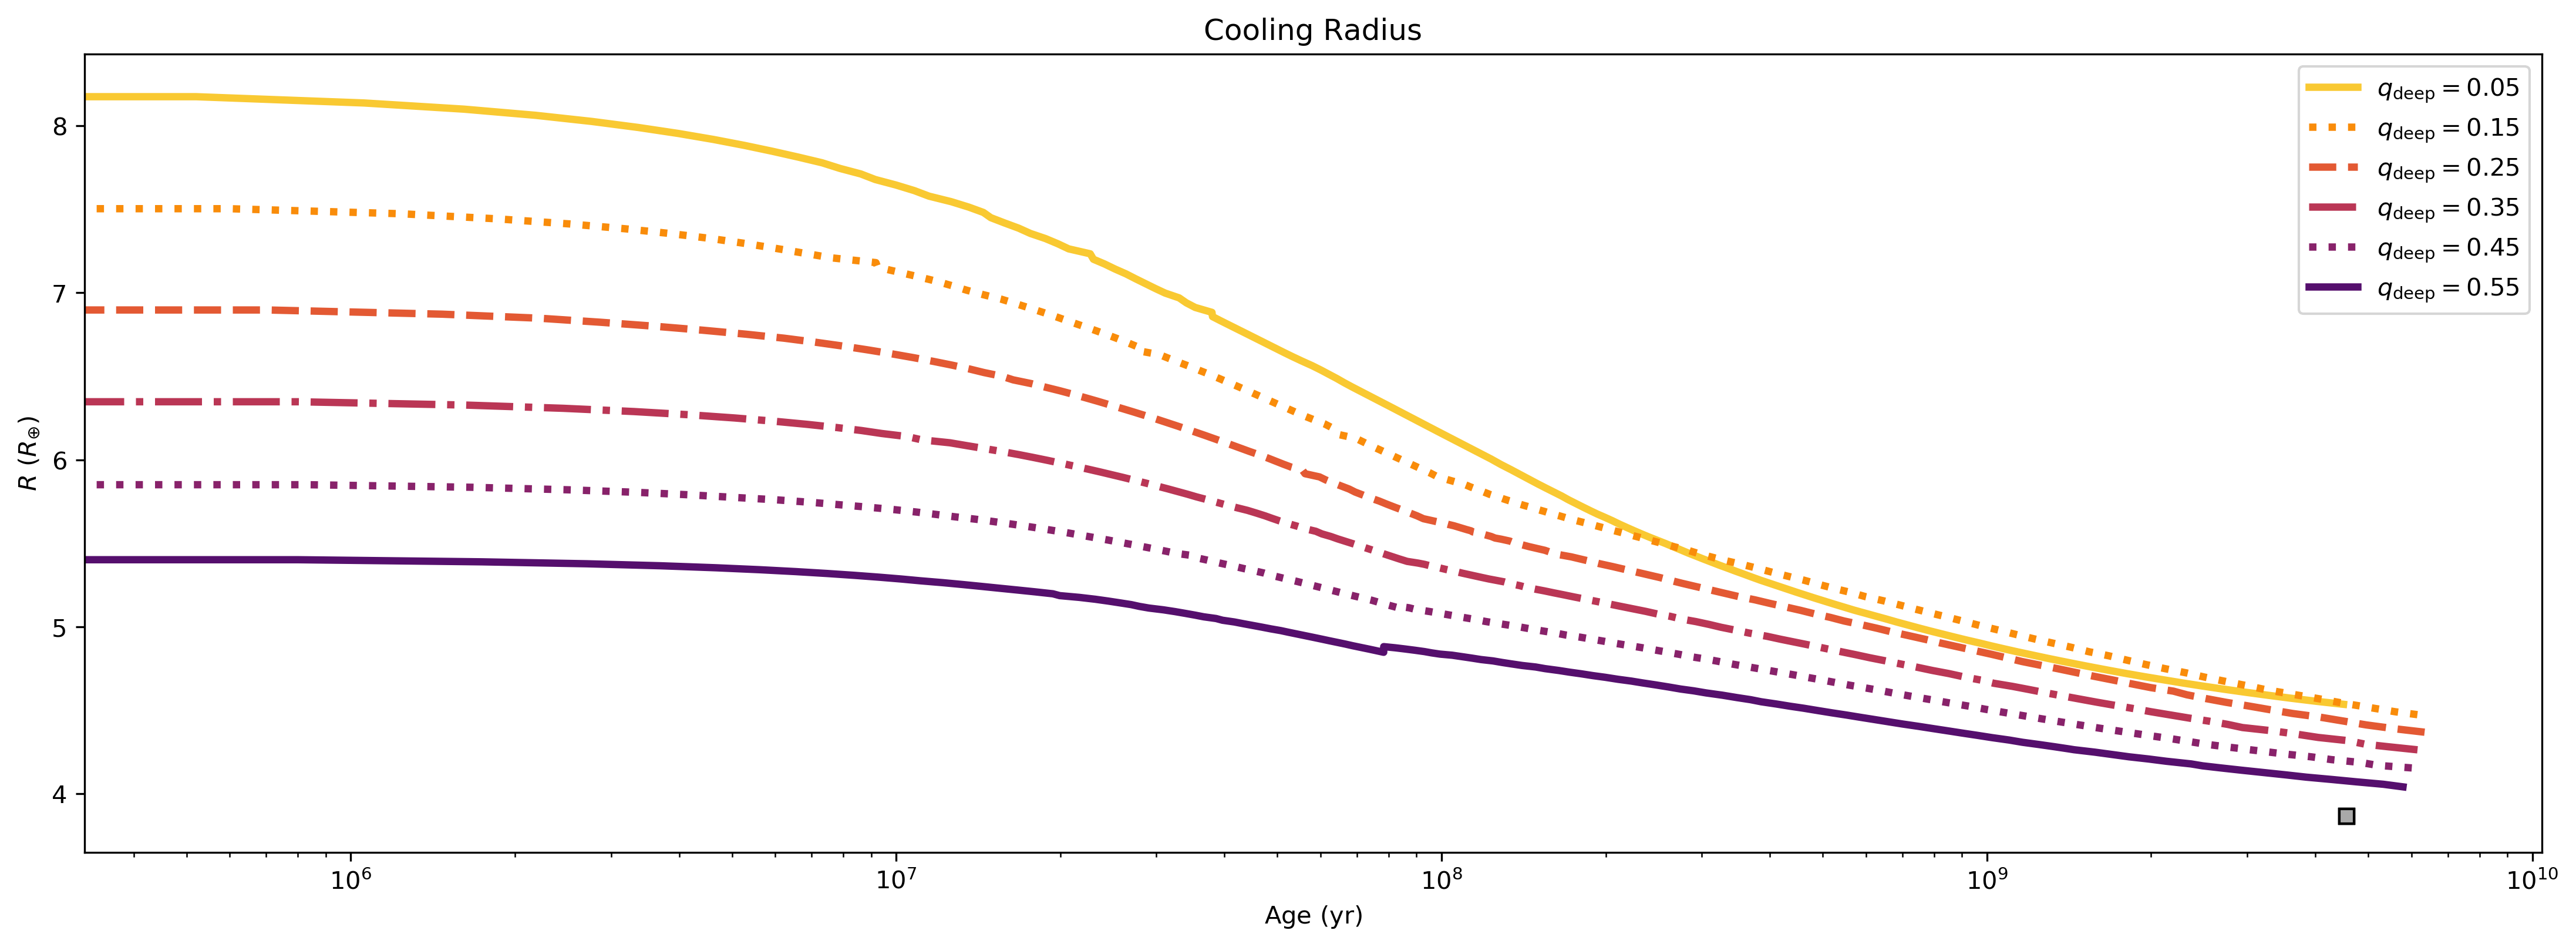
\includegraphics[width=\columnwidth]{figures/n_cooling_radius_nz_4096_logx.png}
 }
\caption[Thermal Evolution Curves for Neptune - Radius]
{As in Figure \ref{fig:evolve_uranus_radius}, but for Neptune.}
\label{fig:evolve_neptune_radius}
\end{figure}



\chapter{Discussion}
We have investigated the impact of condensation and the formation of stable water condensation zones on the thermal evolution of our solar system ice giants. It has been speculated that such thermal boundary layers could act as an imperfect insulator, trapping heat below and allowing the envelope above the boundary layer to cool more rapidly \citep{nettelmann_2016,friedson_2017,leconte_2017,podolak_1991,2019A&A...632A..70S}. It seems plausible that such interiors could explain the problem with Uranus appearing to have no intrinsic temperature. 

While our analysis suggests that moist-adiabatic interiors have a significant impact on the heat flow and thermal evolution of ice giants, making a case for their inclusion in contemporary interior structure models, our findings are nonetheless inconclusive with regard to Uranus's luminosity anomaly. We do find that incorporating a simple moist adiabat, not allowing for the formation of a stable radiative layer, into our interior structure model results in a cooler model Uranus and Neptune than would otherwise be seen with a purely dry model. However, when we allow for the formation of stable radiative layers within the interior, we find in the planet's past a period of rapid cooling within the outer envelope above the radiative layer resulting in a cooler effective temperature at around $7 \times 10^7$ yr. But, the formation of a radiative layer at depth effectively traps heat in the interior, prolonging the the cooling of the deeper interior as we saw previously in Figure \ref{fig:overlay}. As a consequence, both model Uranus and model Neptune eventually become warmer at present time than predicted by either dry or simple moist adiabatic models. 

It is quite possible that reality resembles something in between the binary choice of an atmosphere with a moist adiabat containing a stable thermal boundary layer or an atmosphere with a moist adiabat containing no thermal boundary layer \citep{guillot_2019}. Our assumption of a stable shell of water condensation assumes that there are no other dynamics at play, such as upwelling or entrainment pressure \citep{friedson_2017,2019arXiv190802092G} eroding and punching holes in the stable radiative layer. Such a scenario could plausibly allow for more mixing of the warm gases below and cooler gases above the porous radiative layer. Additionally, if entrainment pressure were to destabilize the radiative layers at earlier, warmer periods in the planet's past, but allowing for stable radiative layers to exist in later, cooler phases, then we might see a period of rapid cooling, similar to those seen in Figures \ref{fig:evolve_uranus_qdeeps} and \ref{fig:evolve_neptune_qdeeps}, but later in time. It is unclear if this would result in a cooler Uranus at present. Efforts are currently underway to determine how long the stable radiative layers exist before being eroded by entrainment pressure, and what impact this may have on thermal evolution.

There are myriad possible actors that influence the cooling trajectories of the ice giants. Radio-occultation measurements from Voyager 2 show that condensation of CH$_{4}$ likely occurs at $ P \approx  1.5$ bar at $T \approx 80$ K \citep{1992AJ....103..967L}. For both ice giants, methane accounts for $15\%$ to $30 \%$ of the atmosphere. Both CH$_{4}$ and NH$_{3}$ exist in abundances that are well above those needed for inhibition of convection \citep{2019arXiv190802092G}. \citep{2020arXiv201204166B} explore possible evidence for composition gradients created by H$_{2}$-H$_{2}$O immiscibility that could inhibit convection. 

Our models were exploratory in nature. As mentioned in Chapter 3, our models converged toward the currently observed radii as we increased $q_{\rm deep}$, the deep water abundance within the outer envelope. Future work should iterate on water abundance within the inner envelope, as well as core mass, in a more consistent fashion. These iterations should produce evolutionary tracks that also match the currently observed radii as well as the $J_{2}$ and $J_{4}$ gravitational moments for a model with a given $q_{\rm deeep}$. We also ignored other uncertainties such as where the ice giants formed within the planetary disk, and their subsequent migratory history.

While water condensation certainly plays a role in the thermal structure and evolution of the ice giants, given their temperature and pressure regimes, future attempts at modeling the ice giants would benefit from including all of these effects.
 

\newcommand{\newblock}{}
\bibliography{wcz_bib}
 

\end{document}
